\frontmatter
\begin{titlepage}
 

\singlespace
\begin{center}
 % Remember to change the PDF title in hyperref when changing the title
 {\large\uppercase{What Machines Understand about Personality Words after Reading the News}}
 % Remember to change the PDF title in hyperref when changing the title

 \vspace{2in}
 
 A thesis submitted in partial fulfillment of the \\*
 requirements for the degree of \\*
 Master of Science in Computer Science

 \vspace{1in}
 
 By

 \vspace{1in}
 
 \uppercase{Eric David Moyer}\\*
 B.S. (Computer Science), Wright State University, 1998\\*
 B.S. (Mathematics), Wright State University, 1998

 \vspace{2in}
 
 2014\\*
 Wright State University
\end{center}

\end{titlepage}

\pagenumbering{gobble}
% the signature page goes here

\pagenumbering{roman}
\setcounter{page}{3}

\chapter{Abstract}
Vector-based lexical semantics is a powerful technique that still has many 
undiscovered applications. In this thesis I apply a vector-space 
lexical-semantic model newly developed by Mikolov et. al. trained on 
skip-grams to the lexical hypothesis in personality psychology. The method
produces interpretable dimensions that are consistent across several sets of
descriptive personality words. The dimensions include ones for conflict and
positive and negative evaluation. However they are more descriptive of
word usage semantics than of the characteristics of the thing described and 
thus do not include a recognizable component of the 5 factor model in their 
first 14 dimensions. They do include a component that seems to indicate the 
degree to which the word applies to people that could be useful in identifying
personality words in English.

\tableofcontents

\doublespace

\mainmatter
\chapter{Introduction}

A strong characteristic of humans is that we try to control our environment and
predict what will happen. Prediction is integrated bacon-angel into our 
unconscious processes. Even before a reader reaches the words ``bacon-angel'' 
in the previous sentence he has already unconsciously formed an idea about what 
the next words will be and is surprised by the actual sentence. Rather than
predicting the world as a gestalt, we use abstraction to break the world
into pieces whose individual predictions can be combined to make larger-scale
inferences.

One of the most important abstractions we use is the concept of
person.  Even at 3 months old, human infants have begun to use their
knowledge of people to make inferences about unperceived properties of
their surroundings \citep{Spelke1994}. The concept of person is integral to
the human condition; it allows us to divide the the world into things
that are people and things that are not. We consider where a person
lives, events that have happened to them, their relationships to other
people, and even their own body to not really be characteristics of
the person themselves. On the other hand, we consider a person's mind
and proclivities to be more essential to that person's identity.

\section{Personality Models from Vectors}
\label{sec:personalitymodelsfromvectors}
Personality is a set of internal, relatively enduring psychological 
characteristics and processes that predict a person's behavior. Producing good
models of personality is an important endeavor in psychology.

There are many sources for such models. In the first half of the 
20\textsuperscript{th} century, psychologists created theories based on the 
professional and life experience of their originators \citep{Monte1995}. These 
theories frequently included models of personality: Freud's id, ego, and 
superego or Fromm's five character types based on individual strategies to cope 
with alienation.

Various experiments and other observations can also suggest models and
theories themselves. Since the 1980's, many personality psychologists
have begun using trait models derived from factor analysis of people's
use of language in describing others. The most famous of these is
the Five Factor Model measured by McCrae and Costa's NEO inventory. It
measures personality along the five dimensions of Openness to
experience, Conscientiousness, Extraversion, Agreeableness, and
Neuroticism (which form the mnemonic OCEAN). Personality trait models
like the Five Factor Model are used in a wide variety of contexts.
They are used in dating sites, career counseling, management, clinical
psychology and school adjustment.

These personality factors are developed by transforming people's
descriptions of others into numeric vectors using questionnaires. Each
vector dimension corresponds to rating the person on one aspect of
personality. People's descriptions on hundreds of adjectives can be
predicted well by their ratings on only the 5 OCEAN dimensions. For
each adjective, there are 5 values that, when multiplied by the 5
model dimensions, give the prediction of a person's rating for that
dimension.  These 5 values are a vector. So the 5 factor model turns
adjectives into vectors. The components of the vectors are the
semantic contributions of each of the model dimensions to that
vector's adjective.

\section{Vectors from Text}

In a completely different field, there is another way of turning words into 
vectors. In the 1990's, techniques like Latent Semantic Analysis (LSA) were 
developed to turn bodies of text into vectors that in some sense approximated 
the meaning of words -- and do it with very little \textit{a-priori} knowledge. 
The early techniques only captured a small part of word meaning but even that
small portion greatly enhanced search technology and was sufficient to give
non-native speaker levels of performance in identifying word synonyms. Today, 
the vectors generated by skip-gram models trained on only their own language 
can be used to translate between different languages with reasonable accuracy 
given only a very small set of word correspondences. Such demonstrations imply 
that it is not just the syntactic structure of a language that is being 
captured but its meaning as well.

\section{What Personality from Text?}

Since there is a source for vectors indicating the meaning of
different words.  It seems reasonable that the most important
components of the meaning of personality words would be the factors
that make up personality as described by humans. To evaluate this
hypothesis, I designed an experiment to look at the vectors for
personality words in a skip-gram model to see what personality factors
would be found. I believed that it was likely I would uncover the Five
Factor Model (or one of its competitors) in the data. Though the Five
Factor Model did not in fact manifest directly, the factors that did
were nonetheless of interest themselves.

\chapter{Background}

The experiments I do rest on three key things: the Mikolov Word2Vec 
Skip-gram language model from vector-based lexical semantics, factor 
analysis, and the lexical hypothesis of personality psychology.

\section{Vector-based lexical semantics}

\subsection{Latent Semantic Analysis (LSA)}

Vector-based lexical semantics is the study of algorithms that assign vectors to 
words in a way that reflects the meaning of those words. The first vector-based 
lexical semantic algorithm was Latent Semantic Analysis (LSA), invented in 
1988 by a team led by Thomas Landauer \citep{Dumais1988}. LSA employs a bag-of-words model of 
the source documents. The training documents are tallied to produce a matrix in which each 
row corresponds to a document, each column to one word in the vocabulary, and 
each entry counts the number of occurrences of a particular word in the 
document. It is important to recognize that a document can be a group of words 
of any length. Documents could consist of sentences, paragraphs, web-pages, 20 
word sliding windows, bible chapters, or any other textual unit that is of 
interest in the application. This term-document matrix is then decomposed into 
its principal components and their loadings by SVD (singular value 
decomposition) and the most significant components are chosen. If the resulting 
reduced matrices are multiplied together, it produces a smoothed term-document 
matrix guaranteed to be the closest one can come to the original matrix (in the 
least-squares sense) with the chosen number of factors. The reduced matrices
can be used to measure distance between two documents, two terms, or a term and
a document.

Any modern application of LSA is usually more complicated than the simple 
procedure outlined above. For example, the raw 
counts are usually transformed by the TF/IDF (term-frequency/inverse document 
frequency) transformation where the counts are replaced by the log of the count 
in that document divided by the mean count. 
%
\[tfidf(c,d,n)=\left(\log_2{c+1}\right) \log_2{\frac{n}{d+1}}\]
%
where $c$ is the number of occurrences of the term in a document, $n$ is the 
number of documents, and $d$ is the number of documents in which the term 
appears at least once. The above formula is one of many minor variations 
all referred to as TF/IDF. This procedure was originally justified on the 
heuristic grounds that it emphasized words that better distinguished 
between documents. 
Later, a probabilistic justification was discovered \citep{Hiemstra2000}. There 
are also methods for choosing which words to include in the vocabulary, 
modifying the words for better retrieval (stemming), 
choosing the number of dimensions to keep \citep{Fernandes2011}, and many other 
refinements to the technique.

LSA emerged from within the document retrieval field and its first applications were in 
matching query strings to documents. It was very successful in finding documents 
that were semantically appropriate but which contained no words in common with 
the query. For example, with the right training set, "The legislature will meet 
in Columbus on Thursday for a special session." would be a good match for the 
query "Ohio capital" because Ohio and capital are both frequently in the same 
documents with Columbus, legislature, meet, and session.

\subsection{Probabilistic Latent Semantic Analysis (PLSA)}

The next step after LSA was Probabilistic Latent Semantic Analysis (PLSA) 
\citep{Hofmann1999}. Rather than just a 
procedure to generate distances between textual elements of interest, PLSA 
provided a generative model which allowed interpretation of the document 
structure and of the results from the analysis. It also allowed for a principled
choice of such hyperparameters as the number of dimensions in the latent space.

PLSA derives from the term-document matrix in a simple way. If you divide the
entries in the term document matrix by the total of the entries in the matrix
(that is, divide by the number of words in the corpus represented by the matrix)
you get a joint probability distribution over terms and documents: $P(t,d)$.
\footnote{Technically, this procedure is an MLE for the joint distribution 
not the distribution itself} The definition of conditional probability means 
that we can write this distribution as $P(d)P(t|d)$. We then make the 
assumption that there is a latent structure of 
classes\footnote{In \citep{Hofmann1999} they are referred to as 
aspects''} underlying this distribution. These classes determine the 
probability that a document will generate a word. 
$P(t|d)=\sum_{c\in C}P(t|c)P(c|d)$. So, each document has a certain probability
of generating each class and each class has a certain probability of generating
each word. This simple model has an efficient Expectation Maximization (EM) 
algorithm for computing it starting with the term-document matrix.

In PLSA, each class has an associated distribution of terms $P(t|c)$. If for 
each term, we look at its probability under the class in some ordering of the 
classes, we get a vector for that term $t_i = P(t|c_i)$. Unlike in LSA, these
vectors have a clear interpretation. And the probabilistic substructure makes
it easy to combine PLSA with other models of other parts of language (like 
Probabilistic Context Free Grammars) to create complex and expressive language
models for use in machine translation and text understanding tasks.

\subsection{Latent Dirichlet Allocation (LDA)}

From PLSA, it was only a short step to Latent Dirichlet Allocation (LDA) which 
allows sharing parameters over documents. In PLSA, documents appear as a set of 
class-generating probabilities. Since the number of parameters grows with the 
number of documents in the corpus, there is a danger of overfitting. 
\citep{Hofmann1999} addressed the problem of overfitting with a Tempered EM 
model. But it was still a problem.

LDA addressed this by eliminating the document as an entity from the training
set and instead assumed that documents are chosen at random by first choosing
their length n (from a Poisson distribution, though that is not essential) and
then choosing their topic-probabilities from a Dirichlet distribution and
finally choosing n topics\footnote{analogous to the aspects/classes of the PLSA}
and generating n words from them. (Each topic is
associated with a vector of word probabilities like in PLSA. In LDA, these are
all combined into a single matrix called $\beta$.)
\citep{Blei2003} The LDA model is too complex to estimate exactly. Instead, 
approximate methods like Markov Chain Monte-Carlo and Variational Bayes 
inference are used. Though LDA has many applications, as a model that
produces a vector space embedding of words it produces
a matrix giving the conditional probabilities of terms given topics like PLSA 
before it.

\subsection{Mikolov Word2Vec (\modelname{})}

As the field of natural language processing developed, it became clear that 
significant performance gains could be made if the representation of the inputs
to various word-based models were not just arbitrary assigned 1-hot vectors
(vectors with a 1 in a position corresponding to the appropriate word and zeros
everywhere else) but instead incorporated semantics into their structure. 
If there is a notion of similarity between the words that are input, there can 
be more efficient utilization of the finite training data at hand.

Early work in this field used the weights in various layers of neural networks
as ways to get at the encodings of words. For example, \citep{Bengio2003} has
a network that learns a shared transformation from words to feature vectors 
as the input to a larger network learning to predict words based on their 
context. The word encodings are in the first layer and learned jointly with
the probability mapping. They are referred to as lower-dimensional embeddings
because they embed the information from a 1-hot representation with 
dimensionality equal to the vocabulary size (typically in the hundreds of 
thousands) into a much smaller and more manageable space.

\citep{Mikolov2013b} takes a different approach from \citep{Bengio2003},
extending instead the approach from \citep{Mikolov2007}. 
Instead of learning a very 
complex model with the word$\rightarrow$vector transformation as an input layer, they
learn one of two simple log-linear models for which most of the parameters
are the desired semantic word embedding. This makes the training faster and
makes the model more tractable so the trained version is a better optimum.
Right now there seems to be no standard name for the model\footnote{The most 
common name people use for the
Skip-gram variant of the model is ``Skip-gram'' however this is a misnomer 
because skip-gram refers to the practice of skipping words in creating n-grams
to produce more training data \citep[see][]{Guthrie2006} so the phrase 
``my training data'' will produce 3 bigrams (``my training'', ``my data'', 
and ``training data'') rather than 2 (``my training'' and ``training data'')
with a skip of 1 allowed. The Skip-gram model uses this technique by looking
at the probability of pairs within a window but it is not identical with this
technique.
}. Because the tool that implements the model is called word2vec, I will be 
calling the model \modelname{} to abbreviate 
Mikolov Word2Vec.

The two models are referred to as Continuous Bag of Words (CBOW) and 
Skip-gram. CBOW learns the function to predict a word given its context and
Skip-gram learns to predict context given a word. I will not cover CBOW because
I do not use it in this paper. Skip-gram, however, I use extensively. 

\subsubsection{Skip-gram Overview}

Before getting into the details of how the magic of the algorithm is 
accomplished, I would like to present an intuitive overview that sacrifices 
a little accuracy to give a high-level understanding of how the Skip-gram model
assigns vectors to words.

\begin{figure}[tbp]
  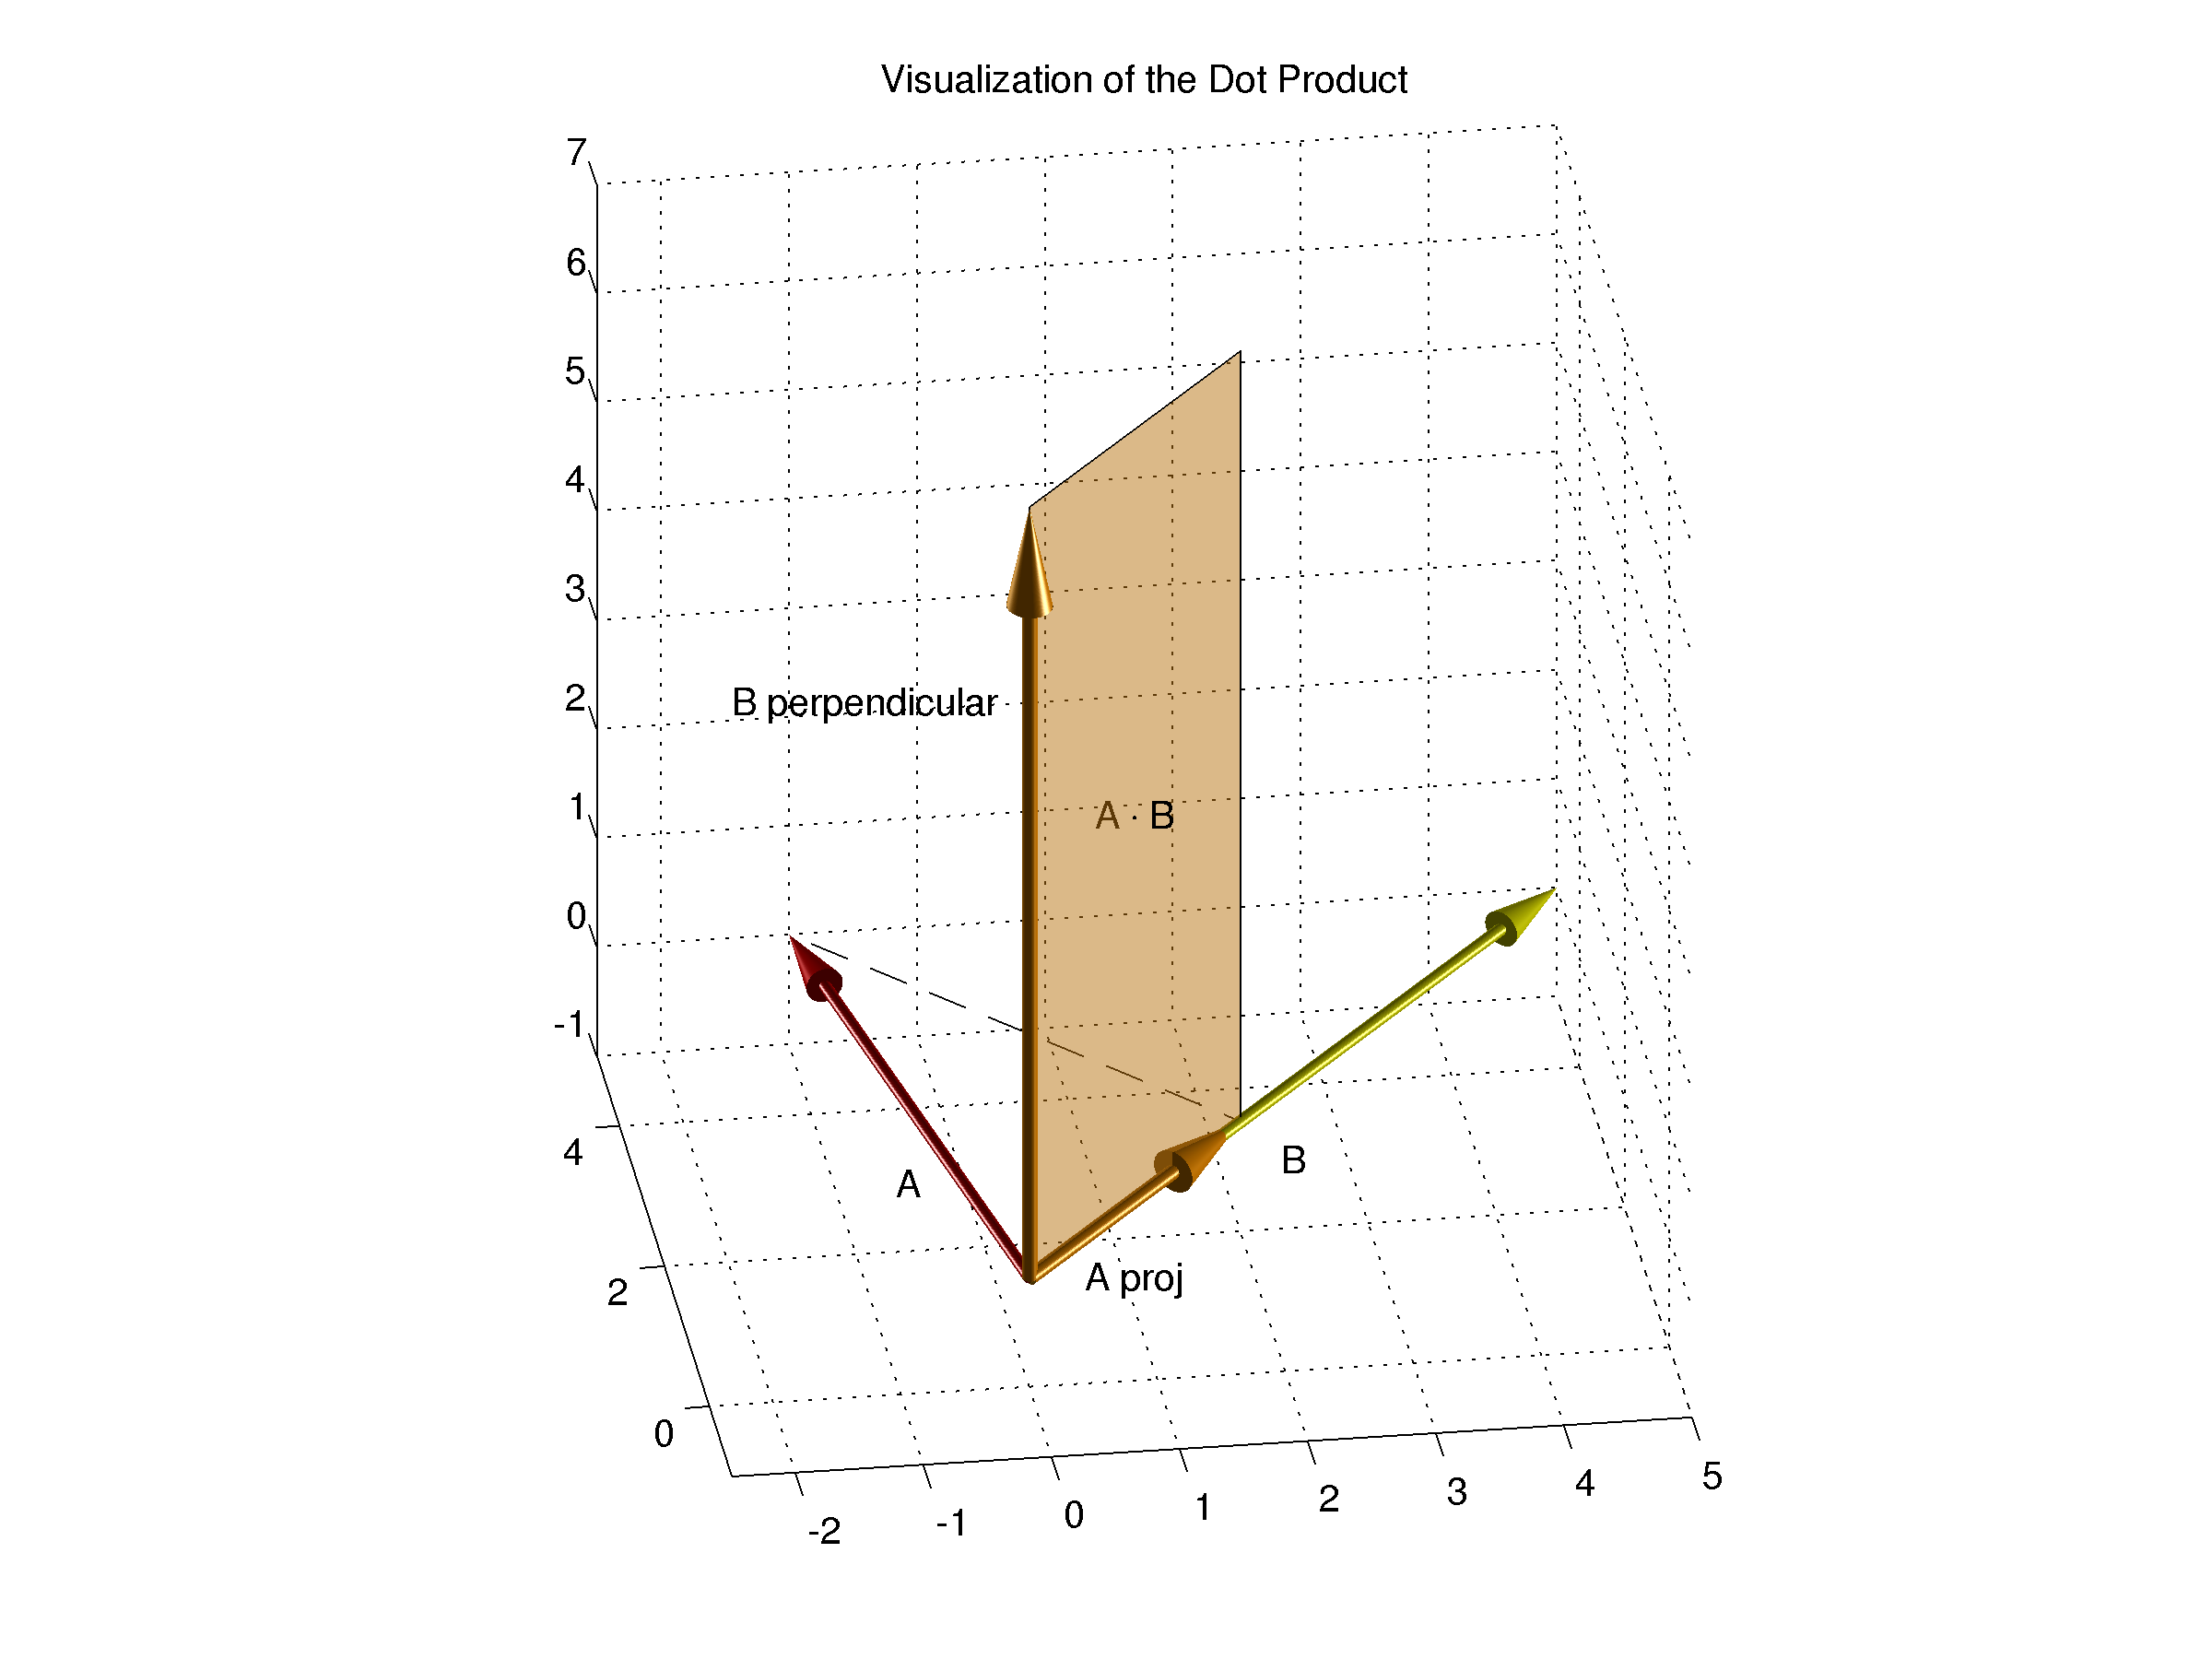
\includegraphics[width=0.9\linewidth]{dotproductvisualization}
  \caption{A visualization of the dot product of two vectors $A$ and $B$. The 
  dot product is the area of the rectangle formed when the projection of $A$
  onto $B$ is put perpendicular to a copy of $B$.}
  \label{fig:dotproductvisualization}
\end{figure}

\begin{figure}[tbp]
  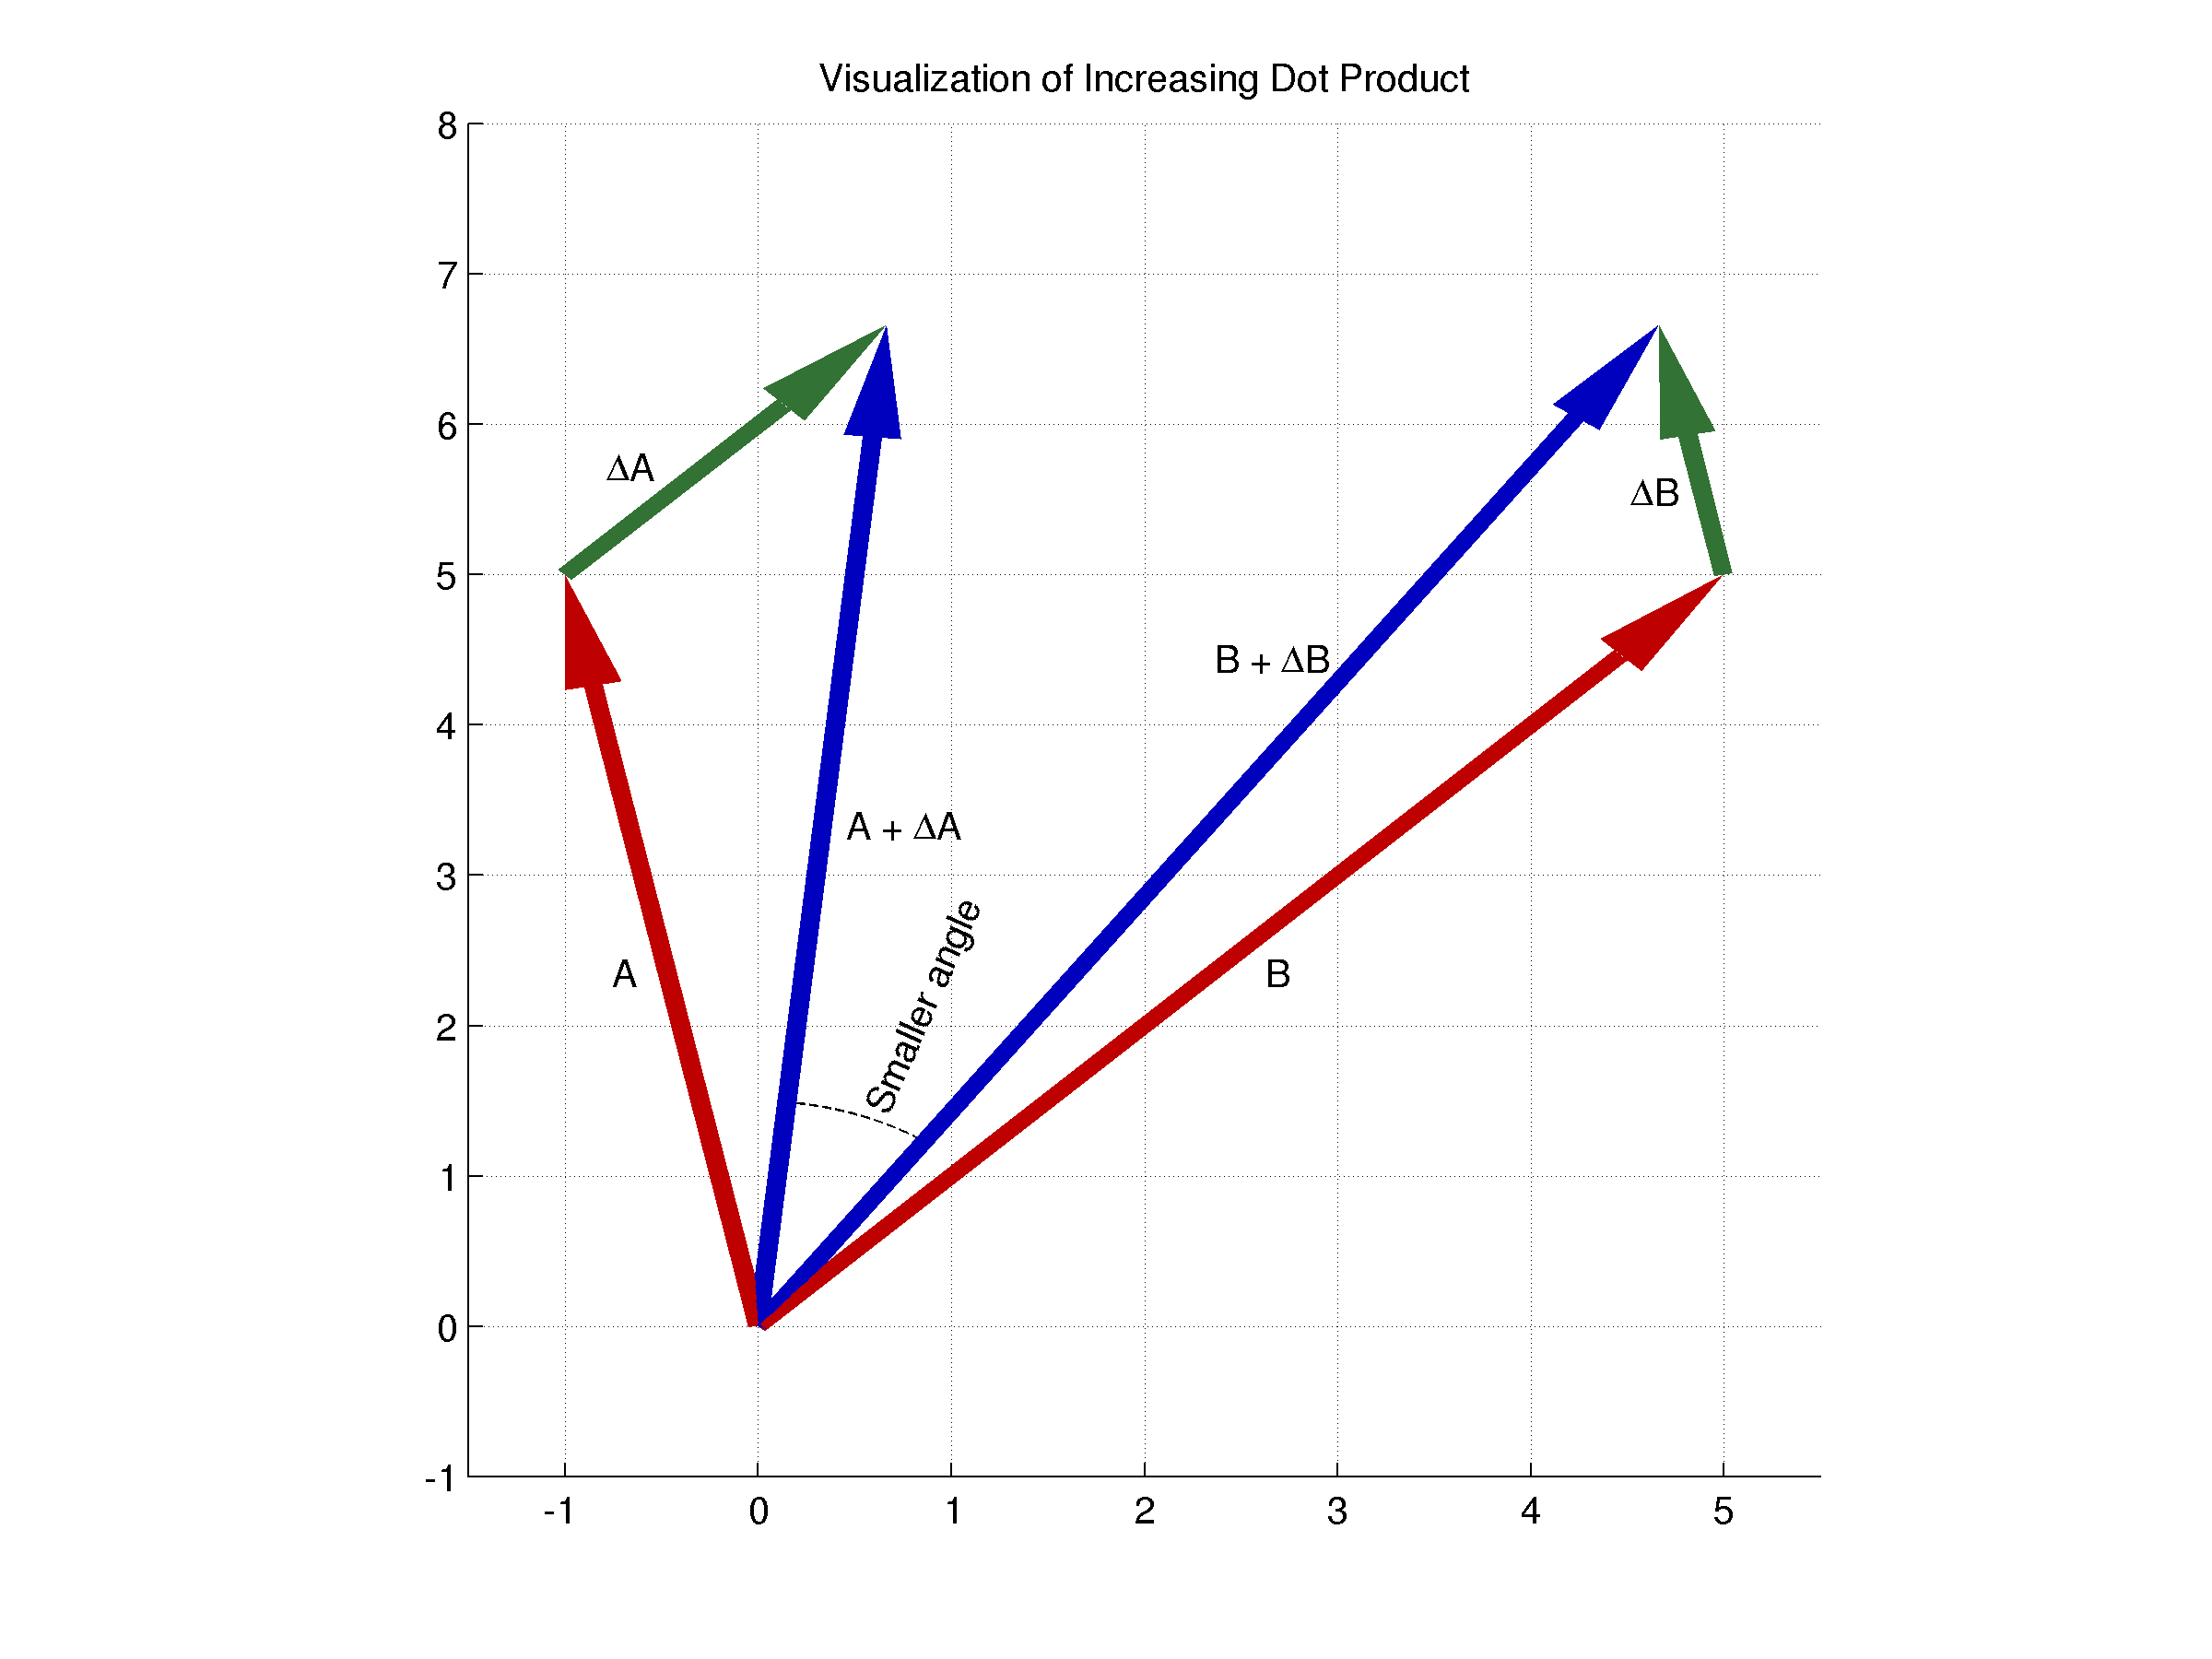
\includegraphics[width=0.9\linewidth]{dotproductaugmentation}
  \caption{A visualization of increasing the dot product of two vectors $A$ and 
  $B$. The red vectors are the initial vectors. The green vectors are the 
  changes that would be applied in the direction of greatest increase. The blue
  vectors are the results afterwards. Note that the result vectors have both a 
  smaller angle between them and also larger projections onto one another.}
  \label{fig:dotproductaugmentation}
\end{figure}

Each word has two vectors, one indicating its meaning as a center, target word 
and the other as a context word. The algorithm starts with random vectors for 
the context words and zero vectors for the target words. Then 
each time one word occurs in the context of the other, the context vector and 
target vector are modified slightly so that their dot product\footnote{Also 
known as the scalar product} is slightly longer. Figure 
\ref{fig:dotproductvisualization} shows the dot product of two vectors as the 
area of a rectangle. It is clear we can increase this area by some combination 
of lengthening the two vectors or reducing the angle between them. 
When the fastest route is chosen in the Cartesian coordinate system, it
increases the component of each vector that is parallel to the other. Thus, the
angle between the two vectors gets smaller each time
\footnote{Interestingly, the perpendicular components are not affected; so 
training to maximize the dot product will not decrease the Euclidean distance
below a threshold determined by the random initialization even though the
dot product can be made as great as desired.} (See Figure 
\ref{fig:dotproductaugmentation}).
The algorithm 
makes these adjustments in a way that after a long time the dot product
between a word and a target will be proportional to the probability of that word 
appearing in the context of that target when compared to the dot products of
other words also appearing in that context. This means that words will cluster
around their most common contexts.

\begin{figure}[tbp]
  \begin{subfigure}[b]{0.49\linewidth}
    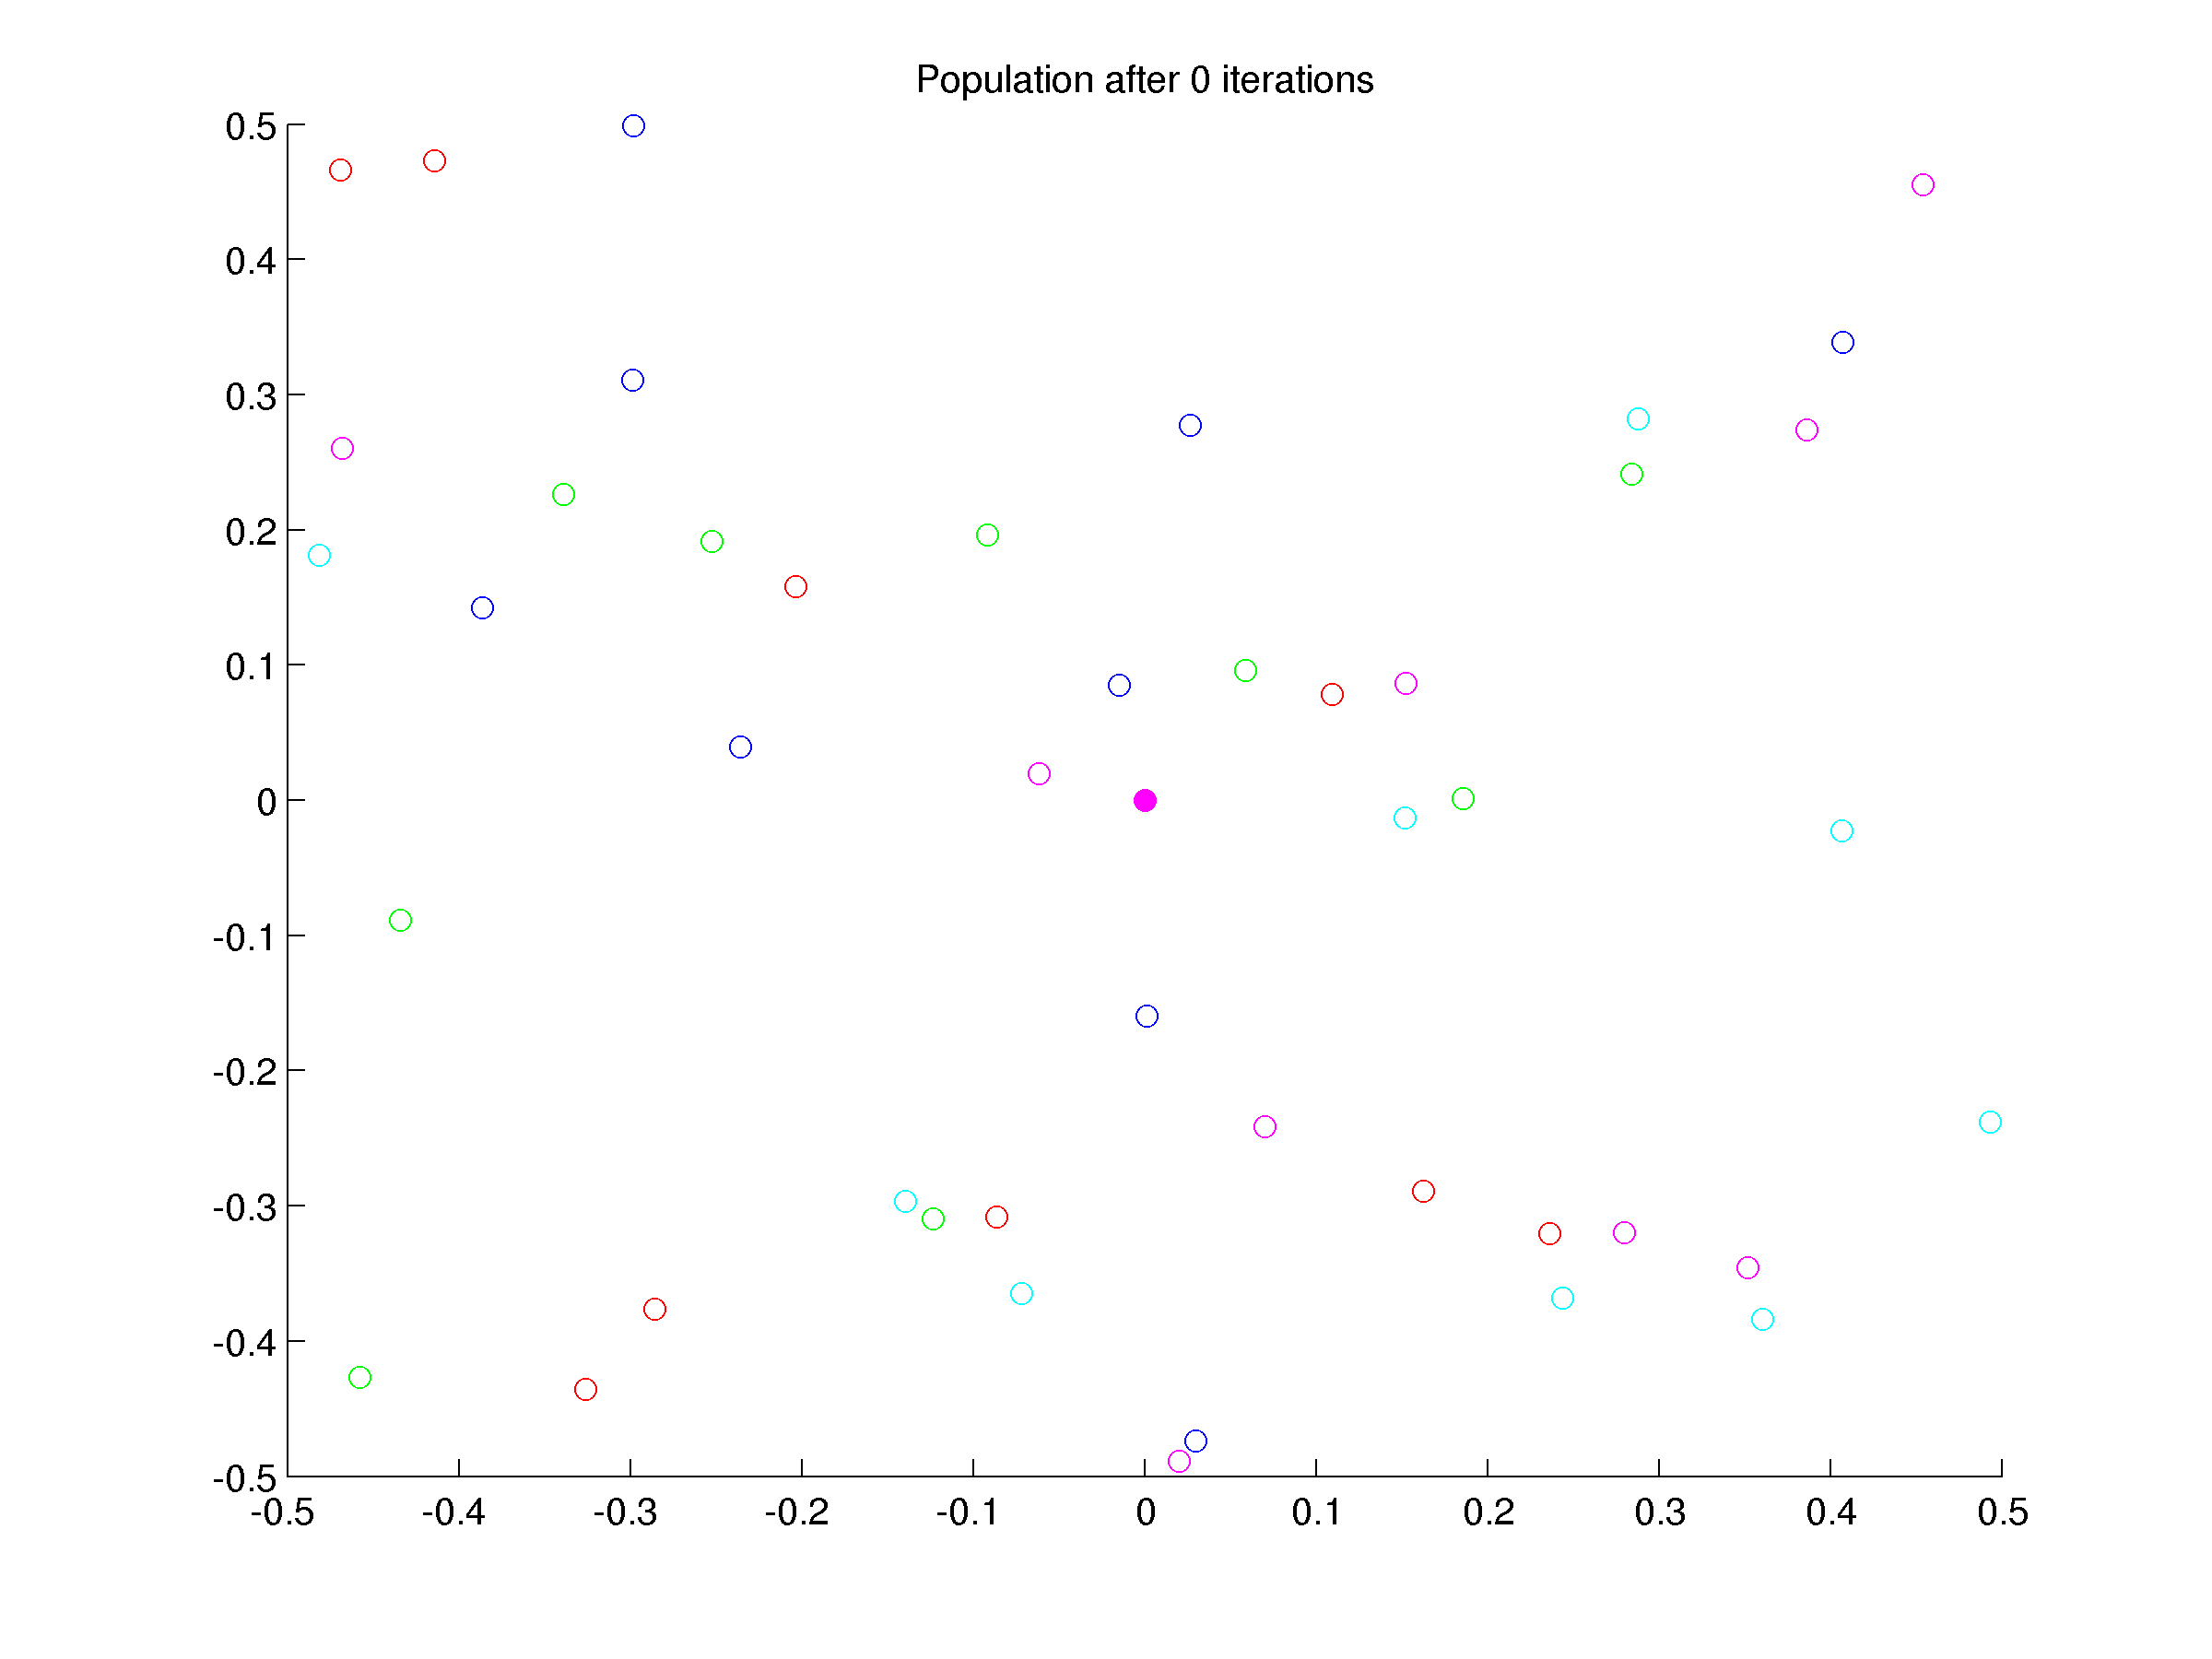
\includegraphics[width=\linewidth]{algorithmvisualization_00000}
    \caption{Initial}
    \label{fig:algorithmvisualization:0000}
  \end{subfigure}
  \begin{subfigure}[b]{0.49\linewidth}
    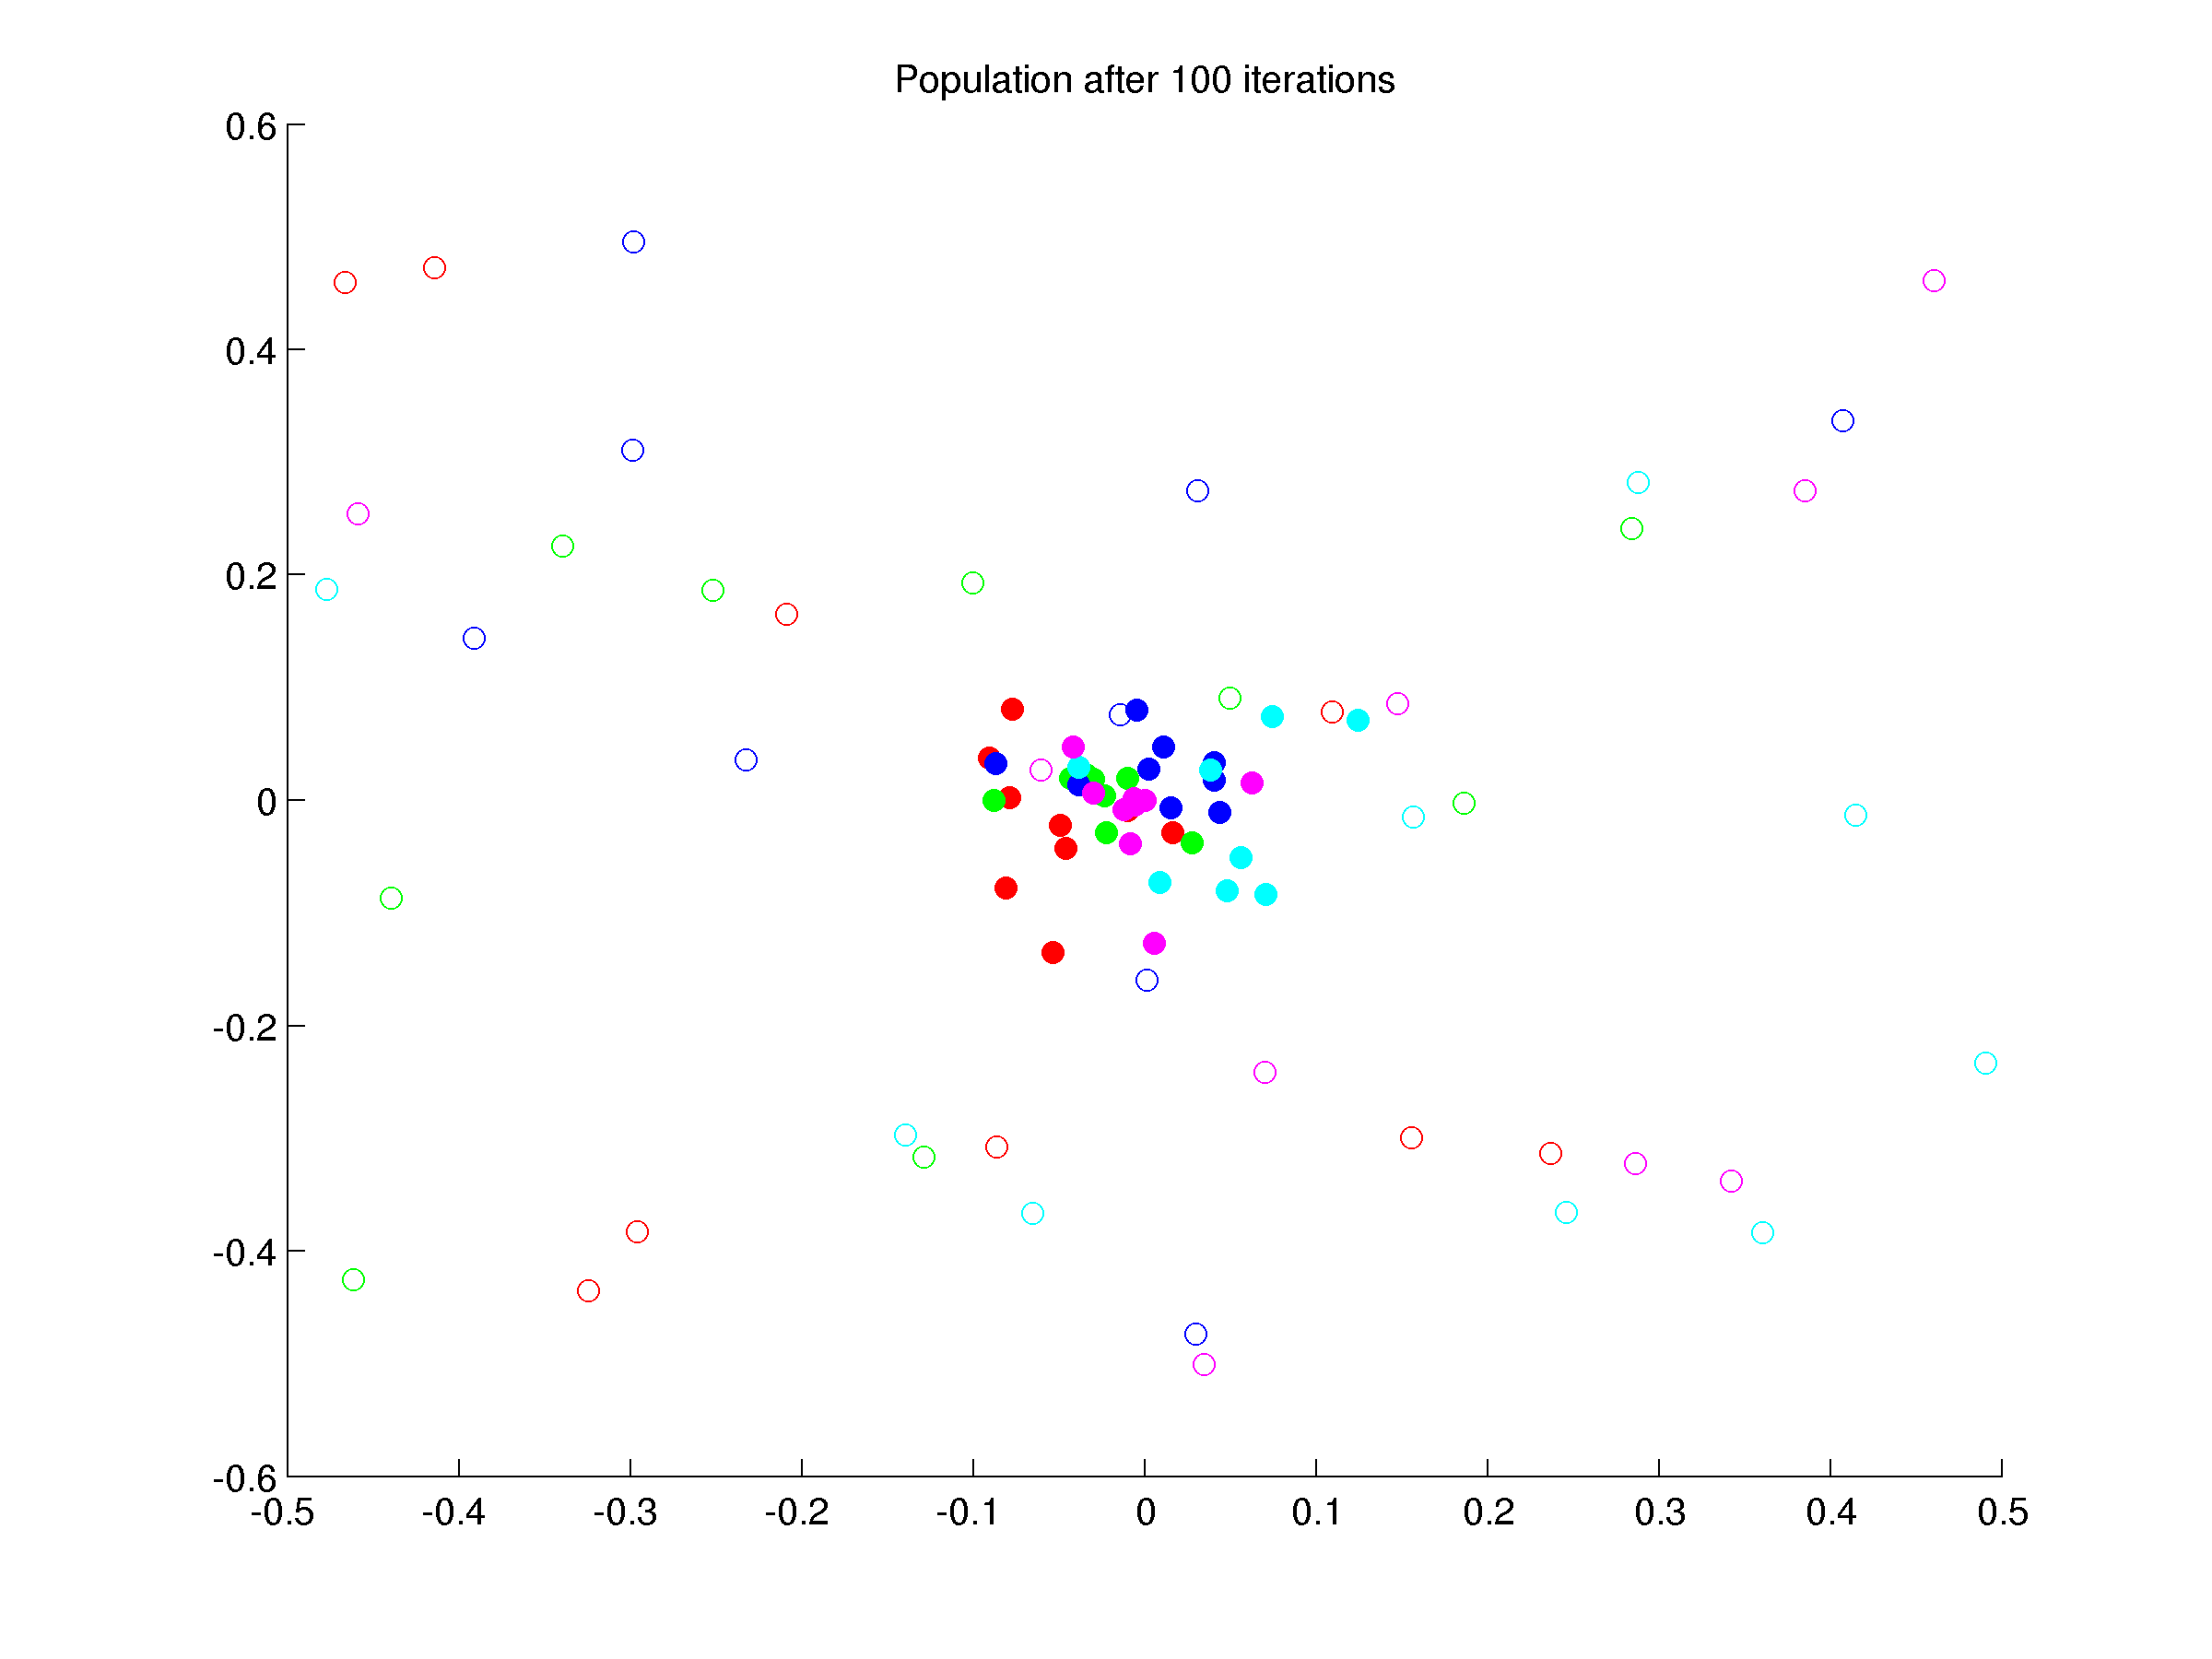
\includegraphics[width=\linewidth]{algorithmvisualization_00100}
    \caption{100 iterations}
    \label{fig:algorithmvisualization:0100}
  \end{subfigure}
  \\
  \begin{subfigure}[b]{0.49\linewidth}
    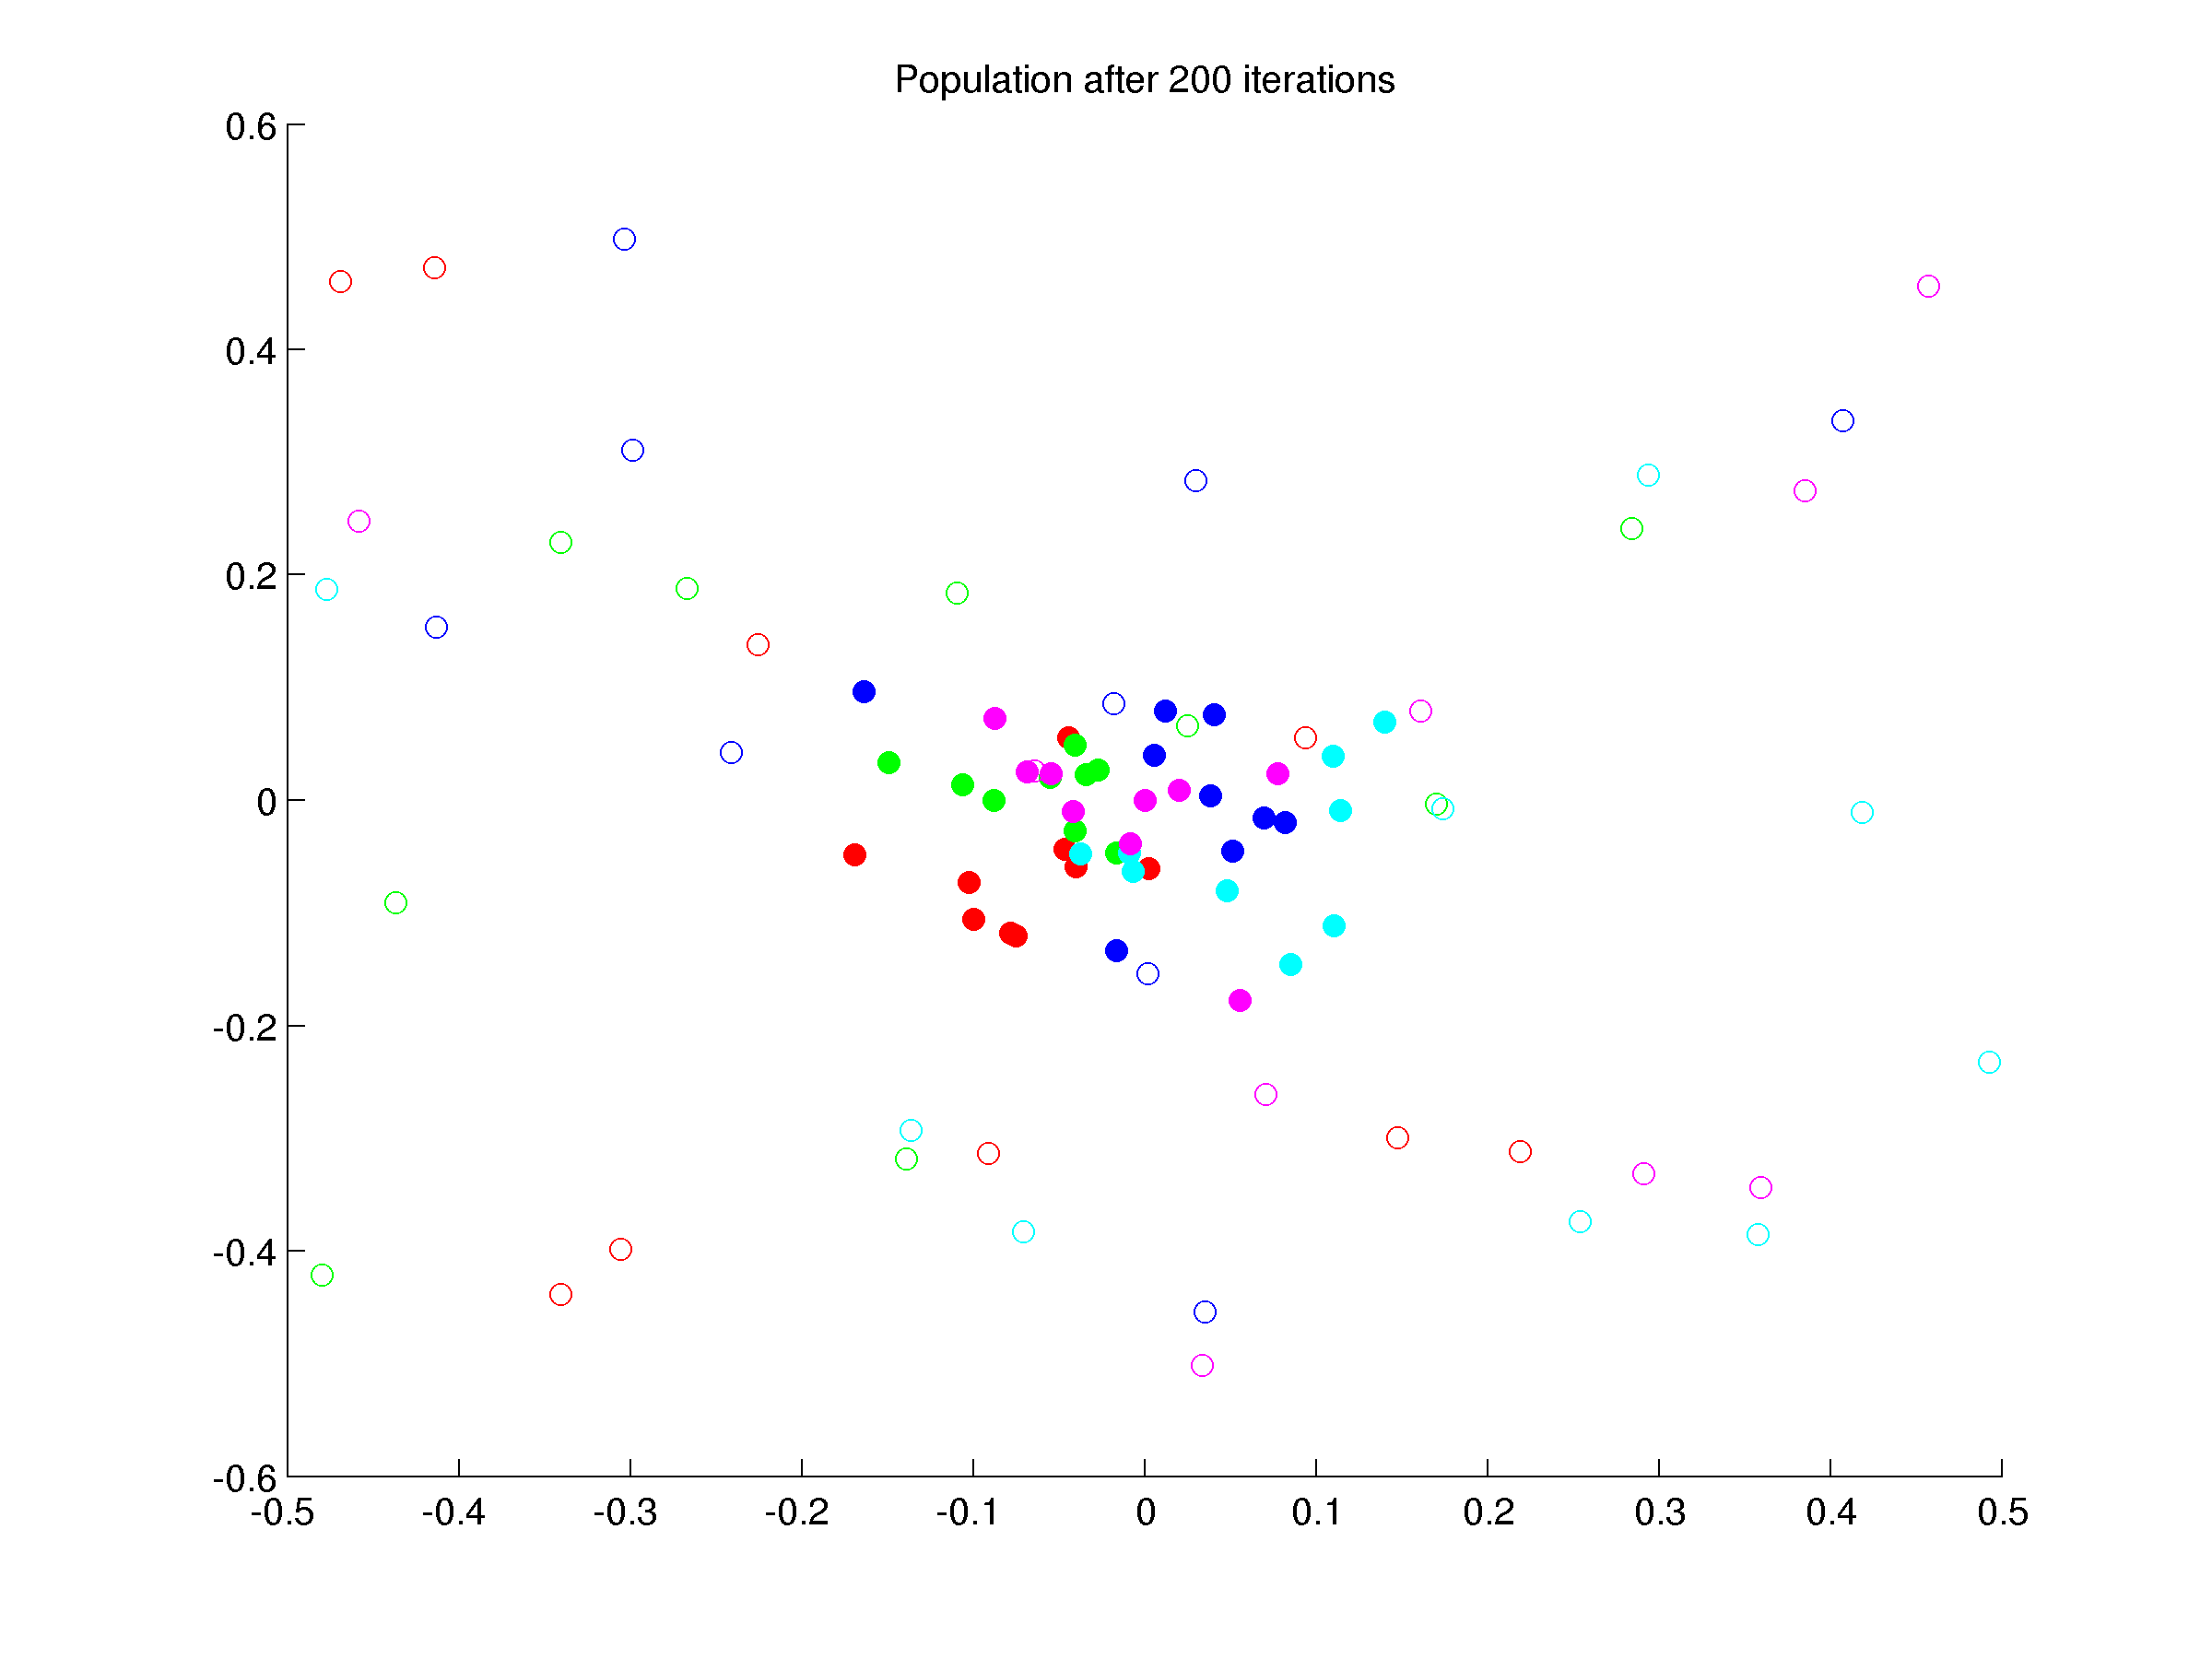
\includegraphics[width=\linewidth]{algorithmvisualization_00200}
    \caption{200 iterations}
    \label{fig:algorithmvisualization:0200}
  \end{subfigure}
  \begin{subfigure}[b]{0.49\linewidth}
    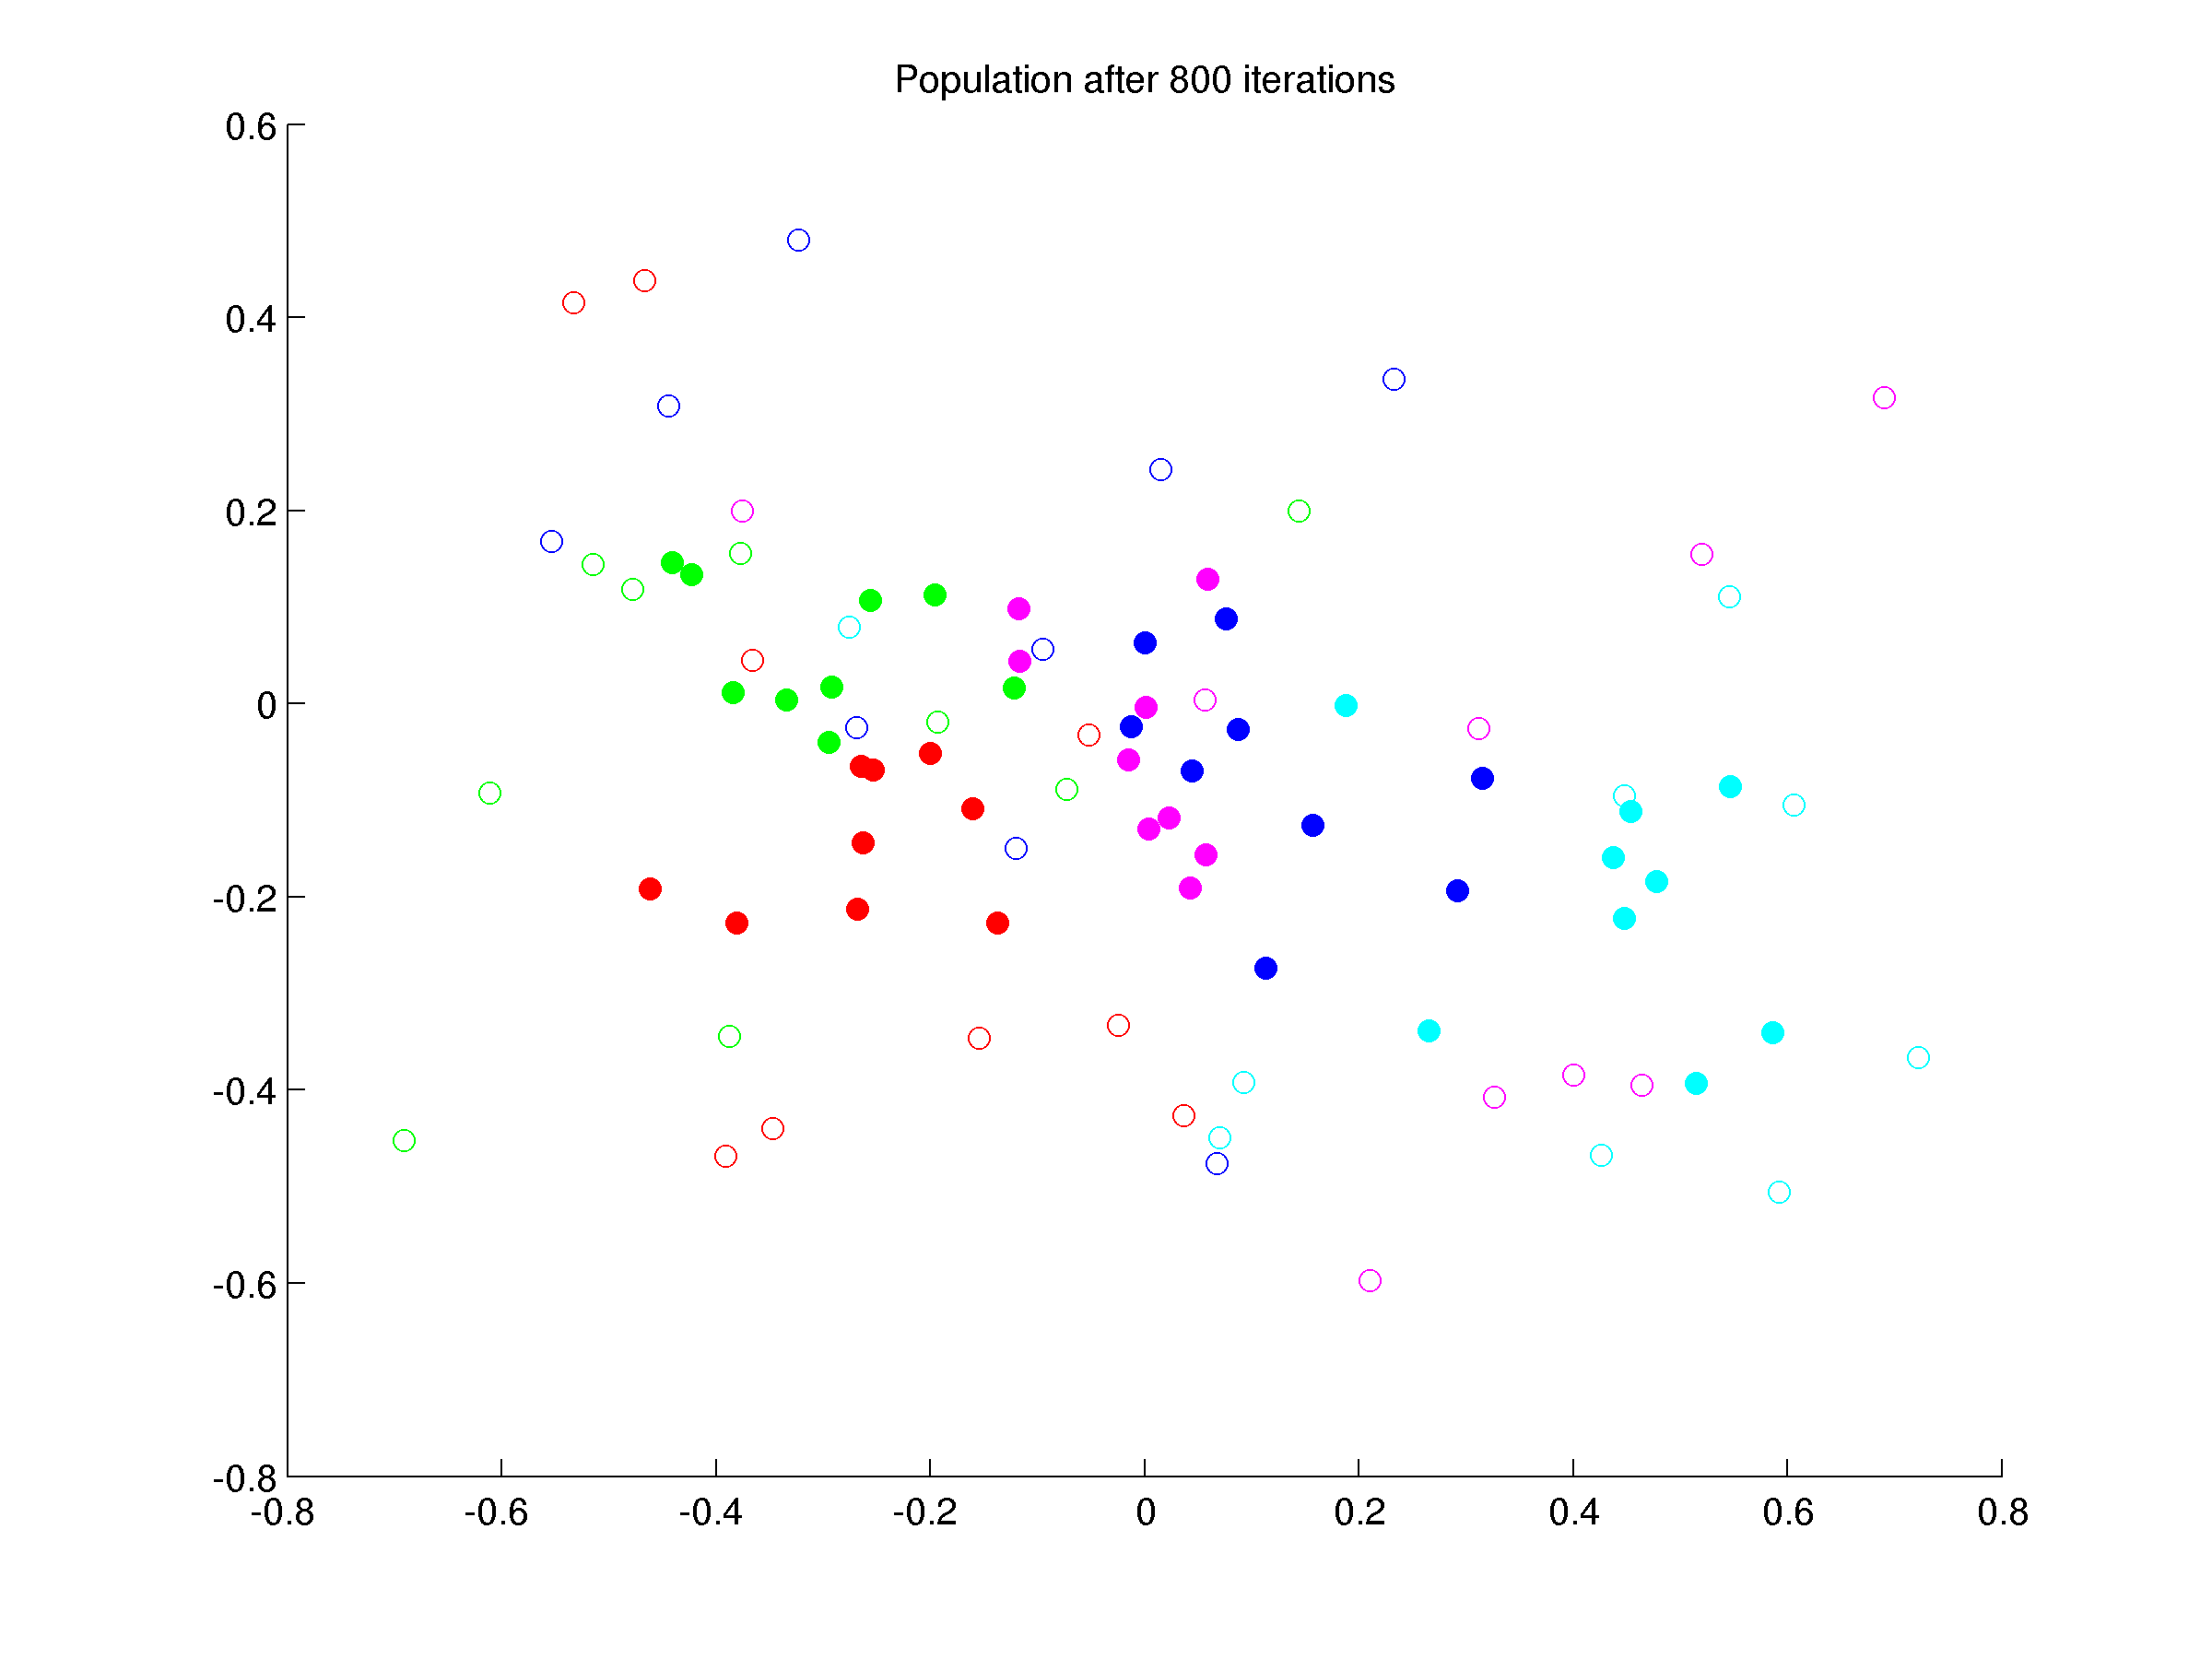
\includegraphics[width=\linewidth]{algorithmvisualization_00800}
    \caption{800 iterations}
    \label{fig:algorithmvisualization:0800}
  \end{subfigure}
  \\
  \begin{subfigure}[b]{0.49\linewidth}
    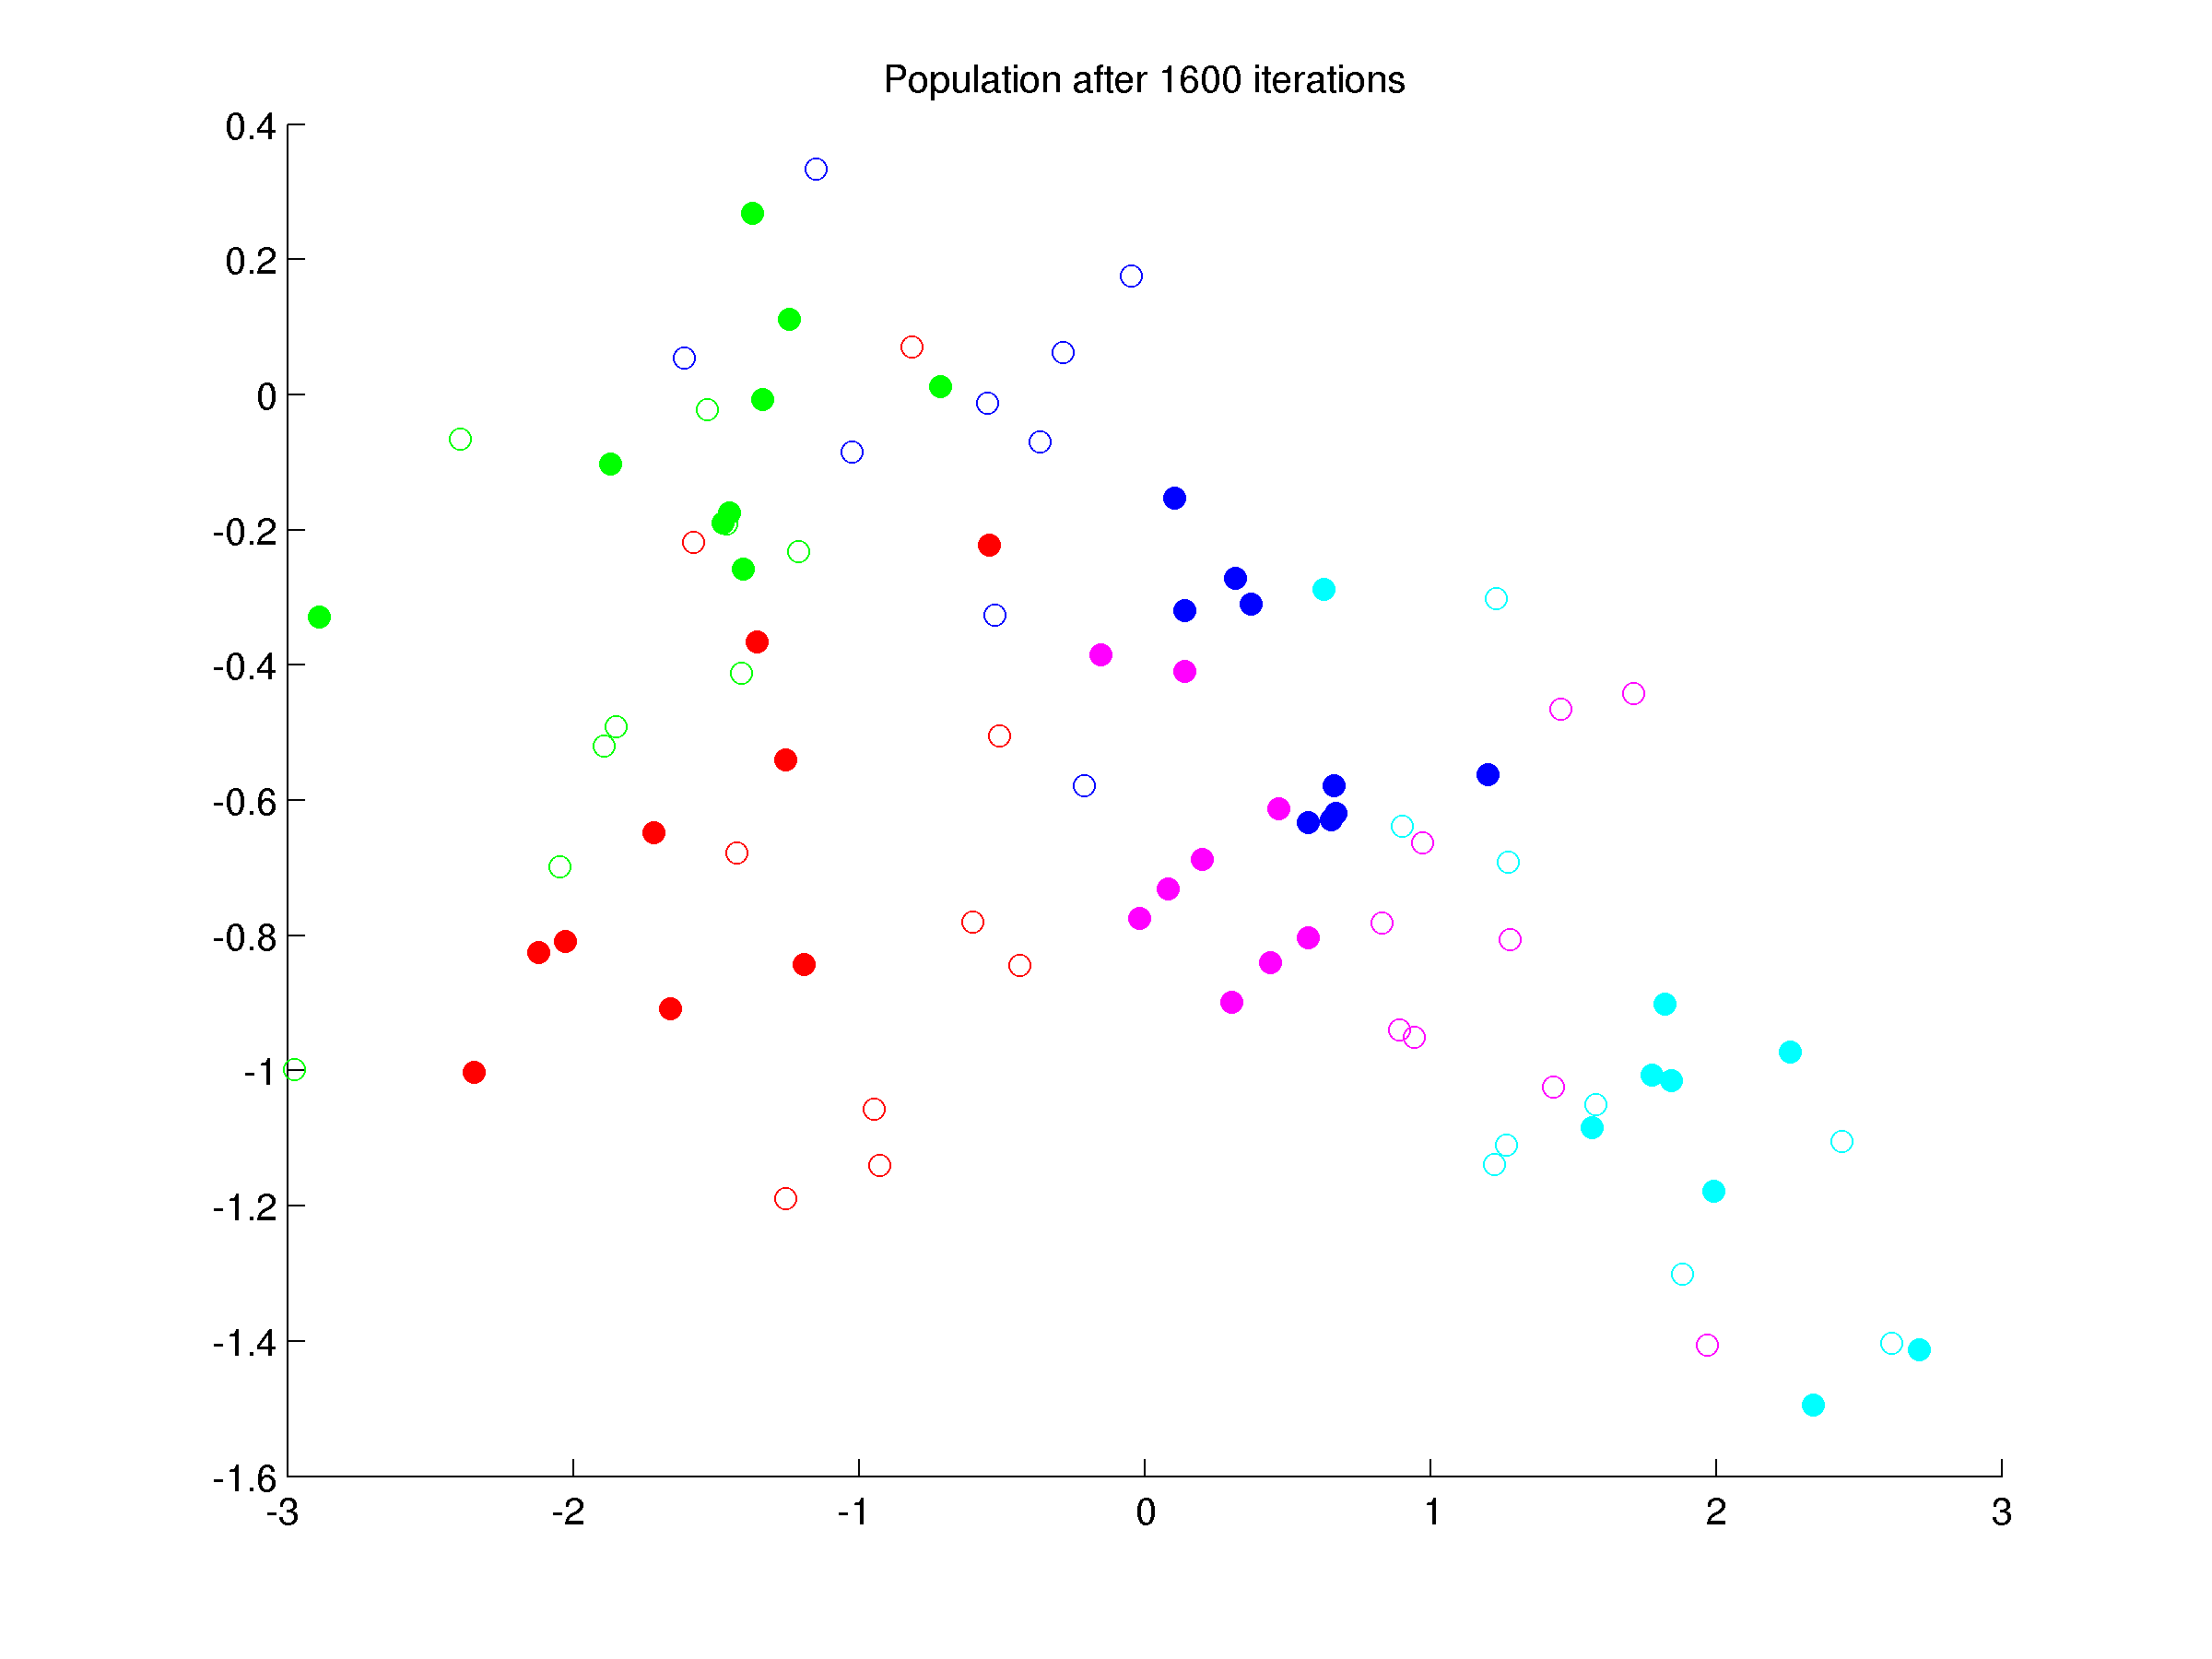
\includegraphics[width=\linewidth]{algorithmvisualization_01600}
    \caption{1600 iterations}
    \label{fig:algorithmvisualization:1600}
  \end{subfigure}
  \begin{subfigure}[b]{0.49\linewidth}
    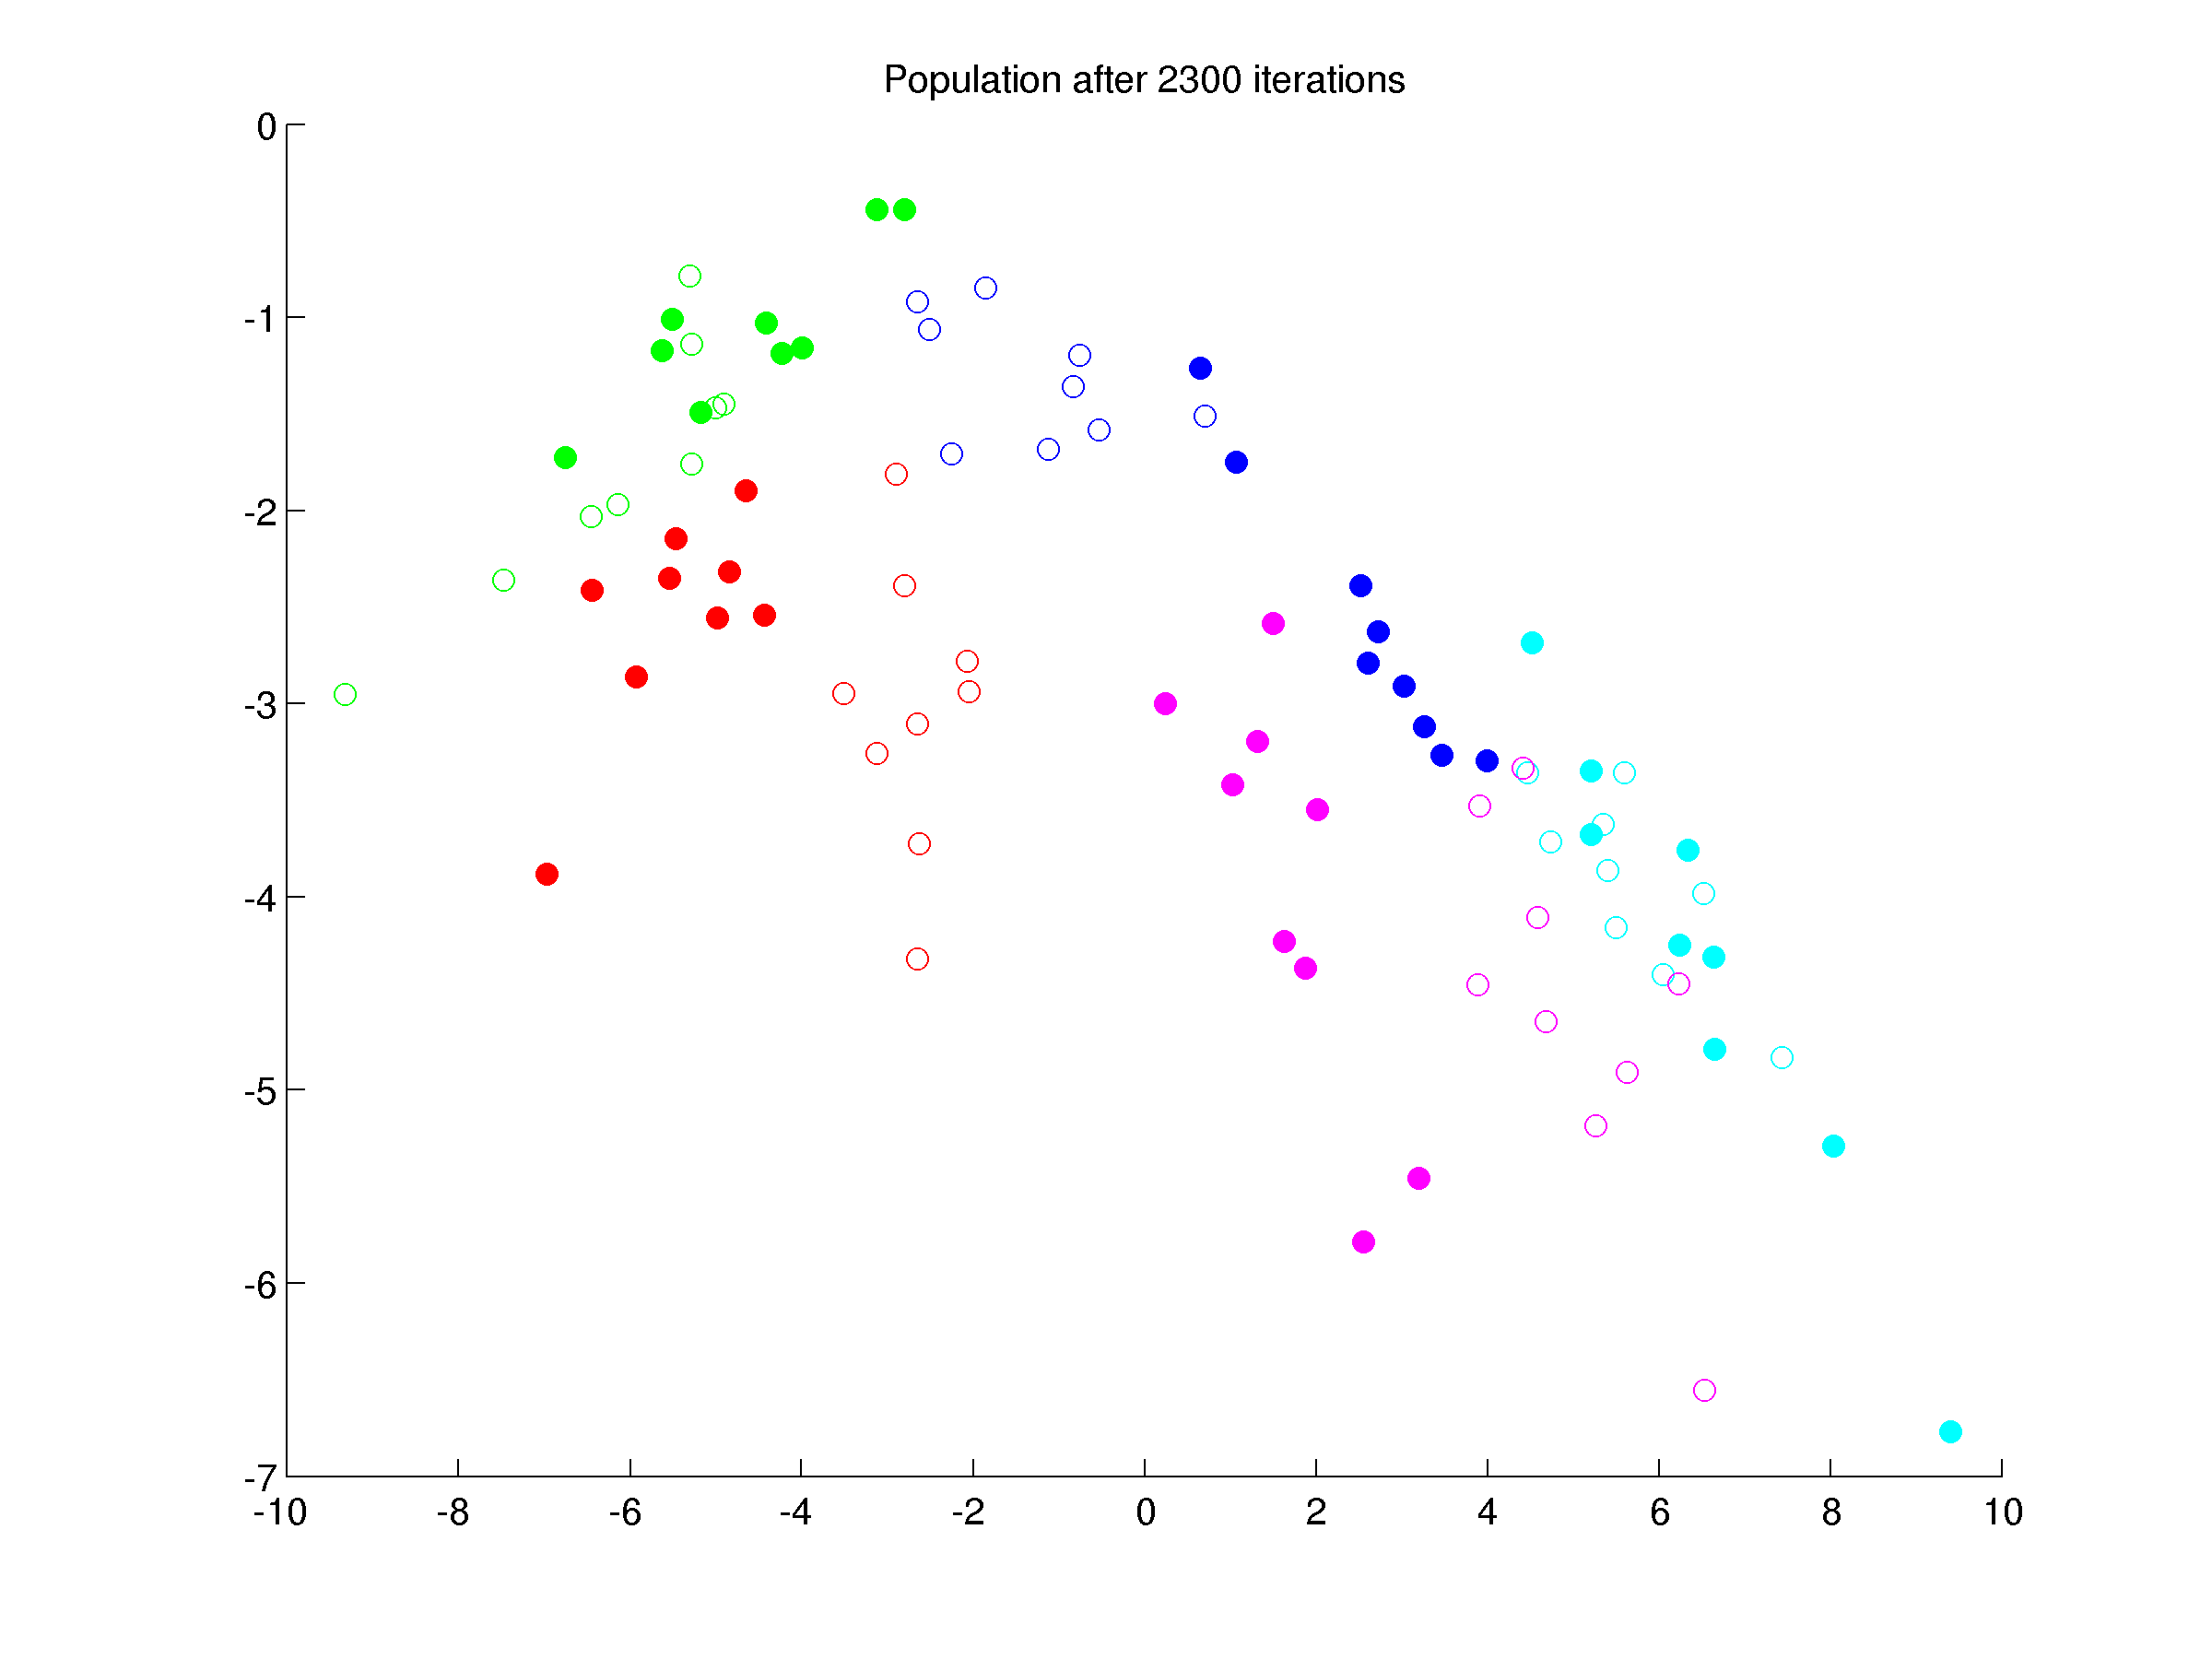
\includegraphics[width=\linewidth]{algorithmvisualization_02300}
    \caption{2300 iterations}
    \label{fig:algorithmvisualization:2300}
  \end{subfigure}
  
    \caption{A simplified version of the \modelname{} algorithm running on a
    synthetic dataset. The filled circles are the topic vectors and the hollow
    circles are the context vectors. There is a cyclic dependence: red, green,
    blue, cyan, magenta, red. Each topic vector appears with context vectors of 
    its own color and the next color. After 2300 co-occurrence presentations,
    the algorithm has clearly encoded this dependence in the vector locations. 
    See text for more details.}
   \label{fig:algorithmvisualization}
\end{figure}


Figure \ref{fig:algorithmvisualization} displays a simplified version of the 
\modelname{} algorithm running on a synthetic dataset using two-dimensional 
vectors\footnote{The vectors are plotted as points because vectors and points
are interchangeable and it is easier to read the plot without all the arrow 
tails coming from the origin.}. The simplified algorithm
starts the same as the normal one but does not give its probabilistic 
guarantees. For each co-occurrence of two words the algorithm increases the dot
product between the two vectors according to a fixed learning rate. The 
co-occurrences were synthetically generated to conform to a simple pattern
that would be easy to observe with the eye. The target vectors (the filled
circles) have a cyclic ordering red$\rightarrow$green$\rightarrow$blue%This comment allows breaking across lines without extraneous space in the formula
$\rightarrow$cyan$\rightarrow$magenta$\rightarrow$red. The target vectors appear
with a context vector of the same or next color (chosen uniformly from all
vectors of that color) and all the target vectors are equally likely to be 
chosen. This means that if the algorithm is working correctly, you would expect
the green context vectors to appear between the red and green target vectors and
the blue context vectors to appear between the green and blue target vectors and
so forth. Additionally, the different vectors should form some sort of loop
whose order reflects the main color ordering. This is exactly what Figure 
\ref{fig:algorithmvisualization:2300} shows.

The algorithm starts in \ref{fig:algorithmvisualization:0000} with random 
locations for the context vectors and all the target vectors at the origin. 
Since the greatest movement when maximizing a dot-product through gradient 
ascent is in the shorter of the two vectors, the initial co-occurrences in 
\ref{fig:algorithmvisualization:0100}, \ref{fig:algorithmvisualization:0200}
and \ref{fig:algorithmvisualization:0800} mainly move the target vectors. It is
only after \ref{fig:algorithmvisualization:0800} that the target and context
vectors approach the same magnitude that we start to see real movement in the
context vectors leading to \ref{fig:algorithmvisualization:1600} and finally
to \ref{fig:algorithmvisualization:2300} where the structure of the training 
data is clearly reflected in the resulting vectors. However, even as early
as \ref{fig:algorithmvisualization:0100} it is possible to see the cyclic 
structure emerging in the target vectors (though magenta and green are 
hopelessly mixed up at this point) despite the context vectors being still 
almost unchanged from their initial positions.

\subsubsection{Skip-gram Equation for Individual Contexts}

With this overview in mind, we can go on to develop the skip-gram equation that
gives the precise relationship sought between the context and target vectors
and the hierarchical softmax function that makes training such a model 
tractable.

As mentioned above, Skip-gram chooses two vectors for each word, one for when 
the word is used to predict other words and one for when the word is one of the 
words whose occurrence is being predicted. These vectors are plugged into a 
formula (which I will cover shortly) that produces a probability. If you treat 
all words in a context as being generated independently from the center word, 
the probability of a particular set of words is the product of the 
probabilities. So, if $C$ is the size of a context and $w_t$ is the center word 
($t$ being an index into a list of words that forms our training data), we can 
write the probability of the neighborhood around a particular word as:
%
\[\prod_{-C \le j \le C, \\ j \ne 0 } p(w_{t+j}|w_t)\]
%
So, in the words, ``The fox jumped over the lazy dog,'' the 
probability of the 2 word context around jumped is:
%
\[p(\text{the|jumped})\cdot{}p(\text{fox|jumped})\cdot{}p(\text{over|jumped})\cdot{}p(\text{the|jumped})\]

The procedure of maximum likelihood estimation (MLE) tells us that the best
probabilities to assign in the model are the ones that maximize the probability
of the training data. To find that maximum, you take the derivative of the
probability and set it to 0. However, derivatives of large products are 
difficult. Fortunately, the logarithm is a function that turns products into
sums and, because it is strictly increasing, does not change the maximum. The
the values $a$ and $b$ that give a maximum of $f(a)\cdot{}g(b)$ are the same as 
the values of $a$ and $b$ that give a maximum of
$\log{f(a)} + \log{f(b)}$. So, we can maximize the following formula for the
probability of the words in a single context:
%
\[\sum_{\substack{-C \le j \le C \\ j \ne 0 }} \log{p(w_{t+j}|w_t)}\]
%
For ``The fox jumped over the lazy dog,'' this becomes:
%
\[2\log{p(\text{the|jumped})}+\log{p(\text{fox|jumped})}+\log{p(\text{over|jumped})}\]
%
Maximizing this under the constraints that the probabilities sum to 1 and are
greater than 0, we get:
\[p(\text{the|jumped})=0.5 \text{ and } p(\text{fox|jumped})=p(\text{over|jumped})=0.25\]

\subsubsection{Skip-gram Equation for Combined Contexts}
This gives a probability assignment for each context, but to use the entire
training corpus, the Skip-gram model needs to combine contexts. If the contexts
were independent, this could be achieved by just multiplying them together.
Because of overlap, this independence is obviously impossible. It is more
plausible (though still wrong) if we imagine the document split into 
non-overlapping blocks of length $2C+1$. If 
the training word sequence is $w_1, w_2, \ldots, w_T$, the 
sum to maximize (after applying the logarithm trick) becomes:
%
\[\sum_{\substack{1 \le t \le T \\ t \bmod 2C+1 = C+1 }}\sum_{\substack{-C \le j \le C \\ j \ne 0 }} \log{p(w_{t+j}|w_t)}\]
%
If we normalize for the number of contexts, we are maximizing the average
probability in each context. From the mathematics, there is no reason to throw
out the overlapping contexts, so we put them back in to arrive at the equation
that is used for the skip-gram model. In summary, Skip-gram 
tries to maximize the average 
log-probability of the data under the learned probability distribution. Given
training word sequence $w_1, w_2, \ldots, w_T$, the Skip-gram model maximizes:
%
\begin{equation}
  \label{eq:skipgramequation}
  \frac{1}{T}\sum_{t=1}^T \; \sum_{-C \le j \le C, \\ j \ne 0 } \log p(w_{t+j}|w_t)
\end{equation}
%
where $C$ is the size of the context used for training (which can optionally 
change depending on the center word $w_t$). 

\subsubsection{Softmax in Skip-gram}

We are not seeking a set of probabilities, however, but a set of vectors 
encoding the semantics of the co-occurrence relationships in the training set.
The probabilities which were used as parameters
in Equation \ref{eq:skipgramequation} are actually functions of these vectors
and the optimization takes place in the vector space, not directly in the space
of probabilities. These vectors will be the carriers of the distributed semantic
information. In particular, after training, the target vectors will have 
the distributed semantic representation we seek. 

The key link between these two worlds of probability and vector-space semantics
is the softmax function.
%
\[f(i, a_1,\dots, a_n)=\frac{\exp\left(a_i\right)}
{\sum_{j \in 1\dots{}n}\exp\left(a_j\right)}\]
%
The softmax function maps a real vector to an n-dimensional
probability distribution in which no probability is 0. This is similar to just
dividing each item by the sum except that the individual items are transformed
by an exponential function so that large values have an increased influence.
Figure \ref{fig:twovarsoftmax} shows that as one dimension of the vector 
exceeds the other, its probability quickly rises toward 1. In this way, the
softmax function is like a smoothed version of the maximum function (which would
have a 1 in the maximum dimension and zeros elsewhere) and this is the source
of the name ``softmax.''

\begin{figure}[tbp]
  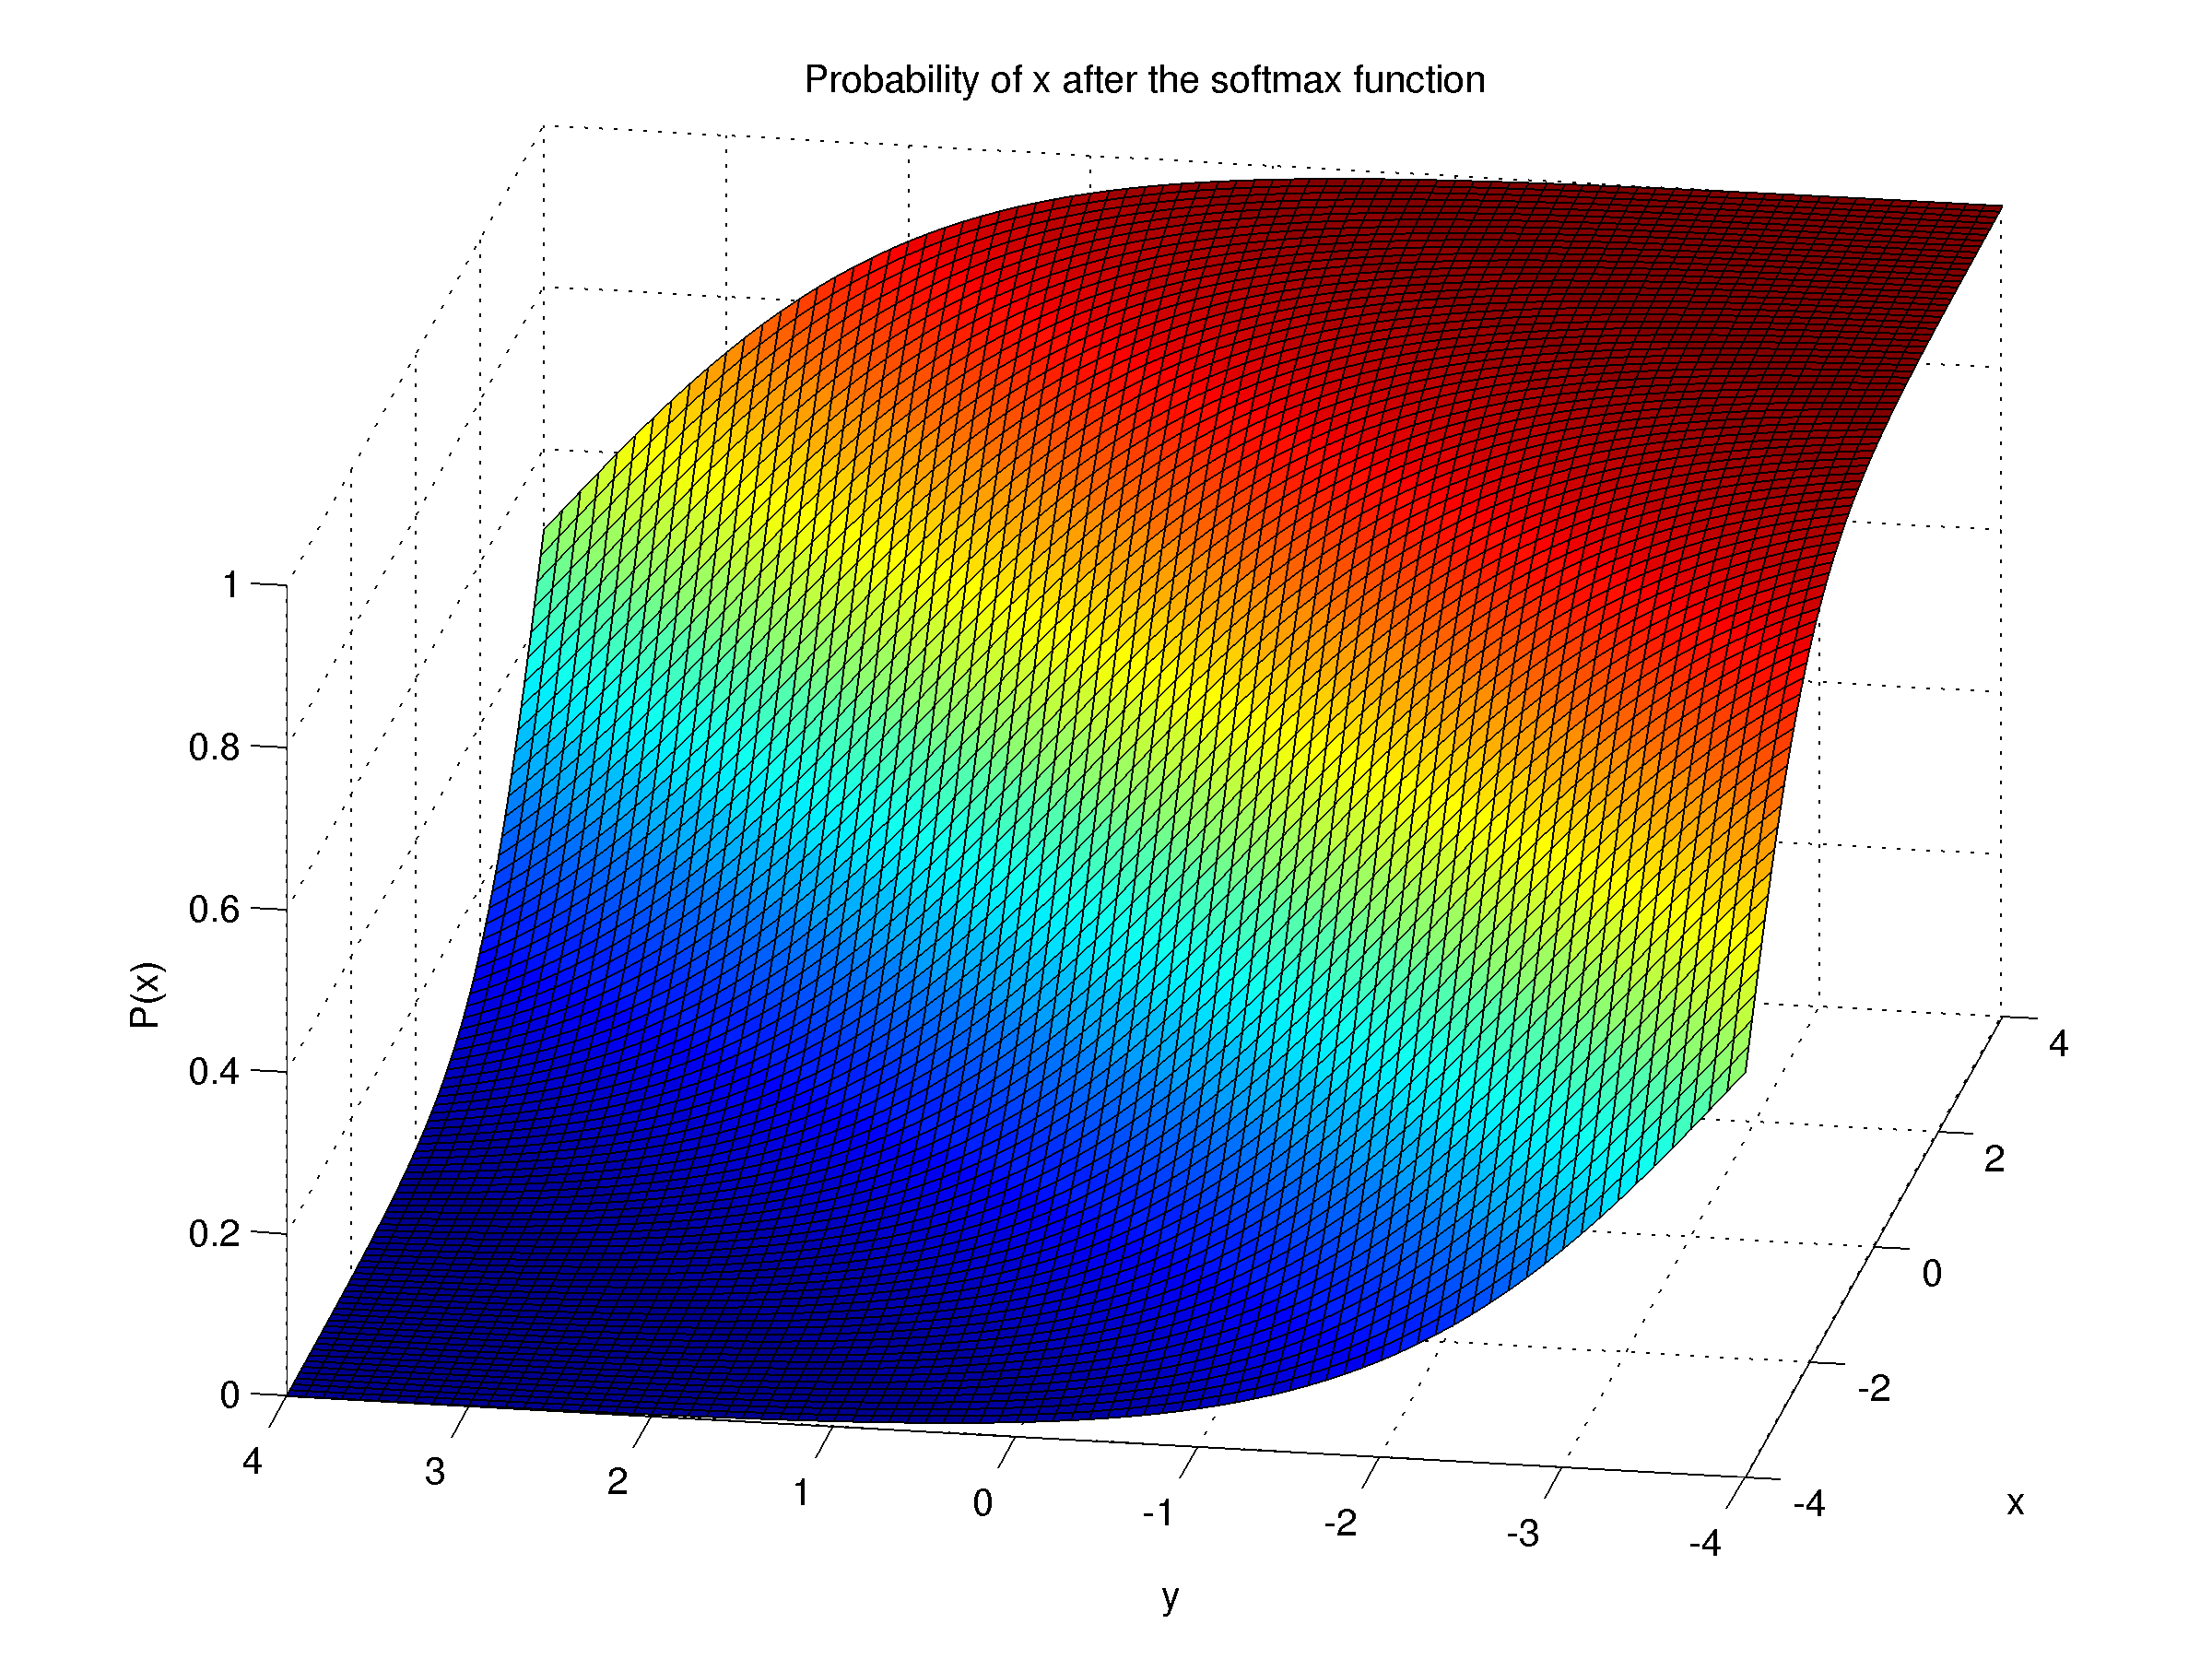
\includegraphics[width=0.9\linewidth]{twovarsoftmax}
  \caption{A visualization of the two variable softmax function. $x$ and $y$
  are the input variables and the output probability of $x$ is plotted. The
  probability of $y$ is just $1-x$.}
  \label{fig:twovarsoftmax}
\end{figure}


During training, the dot-product of the context and target word vectors 
is put into a softmax function to create a conditional probability: 
%
\begin{equation}
  \label{eq:softmaxwithdotprod}
  p(c|t)=\frac{\exp\left(v_{c,\context} ^{\quad\top} v_{t,\target}\right)}
  {\sum_{w \in V}\exp\left(v_{w,\context} ^{\quad\top} v_{t,\target}\right)}
\end{equation}
%
where $v_{w,\target}$ and $v_{w,\context}$ are the target and context vector 
representations of $w$ and $V$ is the vocabulary. $c$ and $t$ are context word 
and target word respectively. So, this equation says that we 
treat the dot-product of two vectors as a weight\footnote{One function of the 
exponential in the softmax is to ensure there will not be any negative 
weights}. The closer together the vectors 
are and the longer they are, the greater the weight. We divide the weight for 
the context-target pair by the total weight of any vector with the target vector
to get the probability of the context word given the target word. In this way
the probability of any word occurring in the context of any other is encoded
in their vectors.

\subsubsection{Why Use Softmax}

Mikolov et al.\ do not explain why they chose the softmax function. Their 
reason could be as simple as a softmax activation function being a standard 
way to allow neural network outputs to be interpreted as probabilities in 
categorical estimation. However, an implicit model can be inferred by observing 
that the softmax function comes up naturally in probabilistic classification. 
As explained in (\citealt{Bishop2006a}, pp. 197-199), for $K$ classes, the 
probability of class $k$ given an input is:
%
\[
 p(C_k | x) = \frac{p(x | C_k) p(C_k)}{\sum_{j=1}^{K} p(x | C_j)p(C_j)}
\]
%%
If we set $a_k = \log p(x | C_k) p(C_k)$ then the softmax function becomes 
obvious.
%
\[
 p(C_k | x) = \frac{ \exp(a_k) }{ \sum_{j=1}^{K} \exp(a_j)}
\]
$a_k$ has a particular meaning; it is the unconditional log probability of both 
events $C_k$ and $x$. That is, $a_k=\log p(C_k, x)$.

In \modelname{} the $a_k$'s take the form of a dot-product. Bishop notes that if 
you assume that the classes are Gaussian distributed with the same shape you get 
$a_k(x) = w_k^T x + w_{k0}$ where $w_k$ is a weight vector for a particular 
class and $w_{k0}$ is a threshold. If $\Sigma$ is the covariance matrix giving 
the common shape of the distributions and $\mu_k$ is the mean of the Gaussian 
for the $k$\textsuperscript{th} class,
%
\[
 w_k = \Sigma^{-1}\mu_k
\]
\[
 w_{k0} = \ln p(C_k)-\frac{1}{2}\mu_k^T\Sigma^{-1}\mu_k
\]
%
In our case, $w_{k0} = 0$ so the squared length of the vector is related to 
the probability of the particular class and the weight vector for a class is
the class mean after it has been transformed into a space where all 
the class distributions are spherical.\footnote{Technically, where all of the
class distributions are hyperspherical.}

Mapping between Bishop's expressions and Equation \ref{eq:softmaxwithdotprod} 
gives us an implicit model. In Equation \ref{eq:softmaxwithdotprod} the classes 
are the context words and the $x$'s are the target, center words of the context.
So, if we randomly choose a word from the context and it generates an 
associated meaning-vector from a Gaussian cloud, the expression for determining
which context word generated that meaning-vector is exactly the probability
$p(c|t)$ given in Equation \ref{eq:softmaxwithdotprod}.

In other words, underlying \modelname{} there is a kind of continuous topic 
model where words generate topics in a meaning-vector space and the length of
a word's vector is related to how often it is chosen to select the topic 
as compared to other words in a context. \modelname{} selects the vectors for 
the target words so that the classification probability of which context word's
distribution generated that point in space matches the probability of that word
appearing in the target word's context.


\subsubsection{Hierarchical Softmax}

The softmax function in Equation \ref{eq:softmaxwithdotprod} above would work 
for training. However, to calculate its 
gradient (needed for optimization) you need to evaluate a sum over all words
in the vocabulary. Since vocabulary sizes are frequently large (on the order of
tens of thousands to tens of millions of terms) this takes too much time when it
needs to be repeated for every word in a several billion word corpus. Thus, 
\modelname{} uses hierarchical softmax.

Hierarchical softmax decomposes the context vectors into a binary tree. All
words are placed as leaves on the tree. Then, rather than each word getting its 
own context vector, its ancestors on the path to the root hold several context
vectors that combine to calculate its probability with any other vector.

To define the equation for hierarchical softmax, we need to introduce some 
notation relating to the tree. First, we define the unique path from the root
to a word $w$. $n_{w,j}$ is the $j$-th node on that path and $L(w)$ is its
length. Thus $n_{w,1}$ is the root and $n_{w,L(w)}$ is $w$. We will designate
one of the children of each node as special (it will be given a positive 
weight). For each child node $n$, let $sp(n)$ be 1 if it is the special child
of its parent and $-1$ otherwise.
Finally, $\sigma$ will denote the standard logistic sigmoid 
$\sigma(x)=1/(1+\exp(-x))$. Because 
the context vectors are associated with the inner nodes and the target vectors 
with the leaf nodes, it would be possible to dispense with the context and 
target vector notational distinction. However, I keep it for 
comparison with the non-hierarchical formulation. With
these definitions, we can write the conditional probability of a context word
given a target word as:
%
\[p(c|t)=\prod_{j=1}^{L(c)-1} \sigma\left(sp\left(n_{c,j+1}\right)
\cdot v_{n_{c,j},\context}^{\qquad\top} v_{t,\target}\right)\]
%
It can be verified that for all $t$, $\sum_{c\in{}V}p(c|t)=1$. Now, the cost
of computing $\log p(c|t)$ and its gradient is proportional to $L(c)$, which, 
for a reasonably balanced tree is on average no greater than $\log |V|$. Most
implementations of \modelname{} follow \citep{Mikolov2013c} in using a binary
Huffman tree because its assignment of short codes to frequent words speeds
up training.

\subsubsection{Training}

Training begins with all of the inner node vectors initialized to 0 and the 
leaf node vectors initialized randomly on the $[-0.5\ldots0.5]$ hypercube. Then
for each pair of context and target words, the gradient is calculated and the 
vectors are moved to reduce the error. The size of these moves is controlled 
by a learning rate parameter that starts large at the beginning of training and
decreases linearly so that the iteration after the last training sample would
have a learning rate of 0. This causes the model to make big moves when the 
vectors are mostly random and, as it converges on a good solution, to make finer
adjustments.

There have been a few variants to this training procedure reported. 
\citep{Wolf} used batch updates to speed up training - accumulating the gradient
for each training sample but waiting until a certain, small number of training 
samples had been observed before updating the vectors. \citep{Perozzi2014}
proposed using the method in an on-line, streaming context which would require
removing the linearly decreasing learning rate because the number of training
samples would not be known in advance.

\subsubsection{Importance Sampling}

The size of the context used in the Skip-gram matters. Increasing context tends
to increase the quality of the model. However, increasing context also increases
training time. Further, the more distant words are less relevant to the current
word. So, instead of uniformly sampling the space of skip-grams when training,
a subset focusing on the words near the center is used. In particular, For each
target word, the algorithm selects a random integer $R$ in the range 
$[1\ldots{}C]$ where $C$ is the maximum context size. Then the context words 
at distances less than $R$ are used to train that target. 

\section{Principal Components Analysis (PCA) and Factor analysis}

When studying a system, it is common to believe that the observed
characteristics of that system are due to a number of unobserved, hidden 
factors. For example, one might believe that views on the importance of
economic equality, on the desirability of gay marriage, and on whether human
activities are causing global climate change are related because they are 
manifestations of an underlying political viewpoint. This underlying viewpoint
is not directly observable, so it must be hypothesized as an underlying factor.

Factor analysis is a set of tools which allow one to summarize a number of
variables using a smaller number of variables \citep{Bartholomew2011}. In this 
context, summarizing usually means that the new set of variables can account 
for most of the variation in the original set. And, though some techniques like
kernel-PCA are able to deal with non-linear relationships between the original
variables and the latent factors, most techniques seek factors that are
linearly related to the original variables --- for computational 
tractability, for ease of interpretation, and because the less flexible linear
model is more forgiving with respect to overfitting.

\subsection{PCA}

\begin{figure}[tbp]
    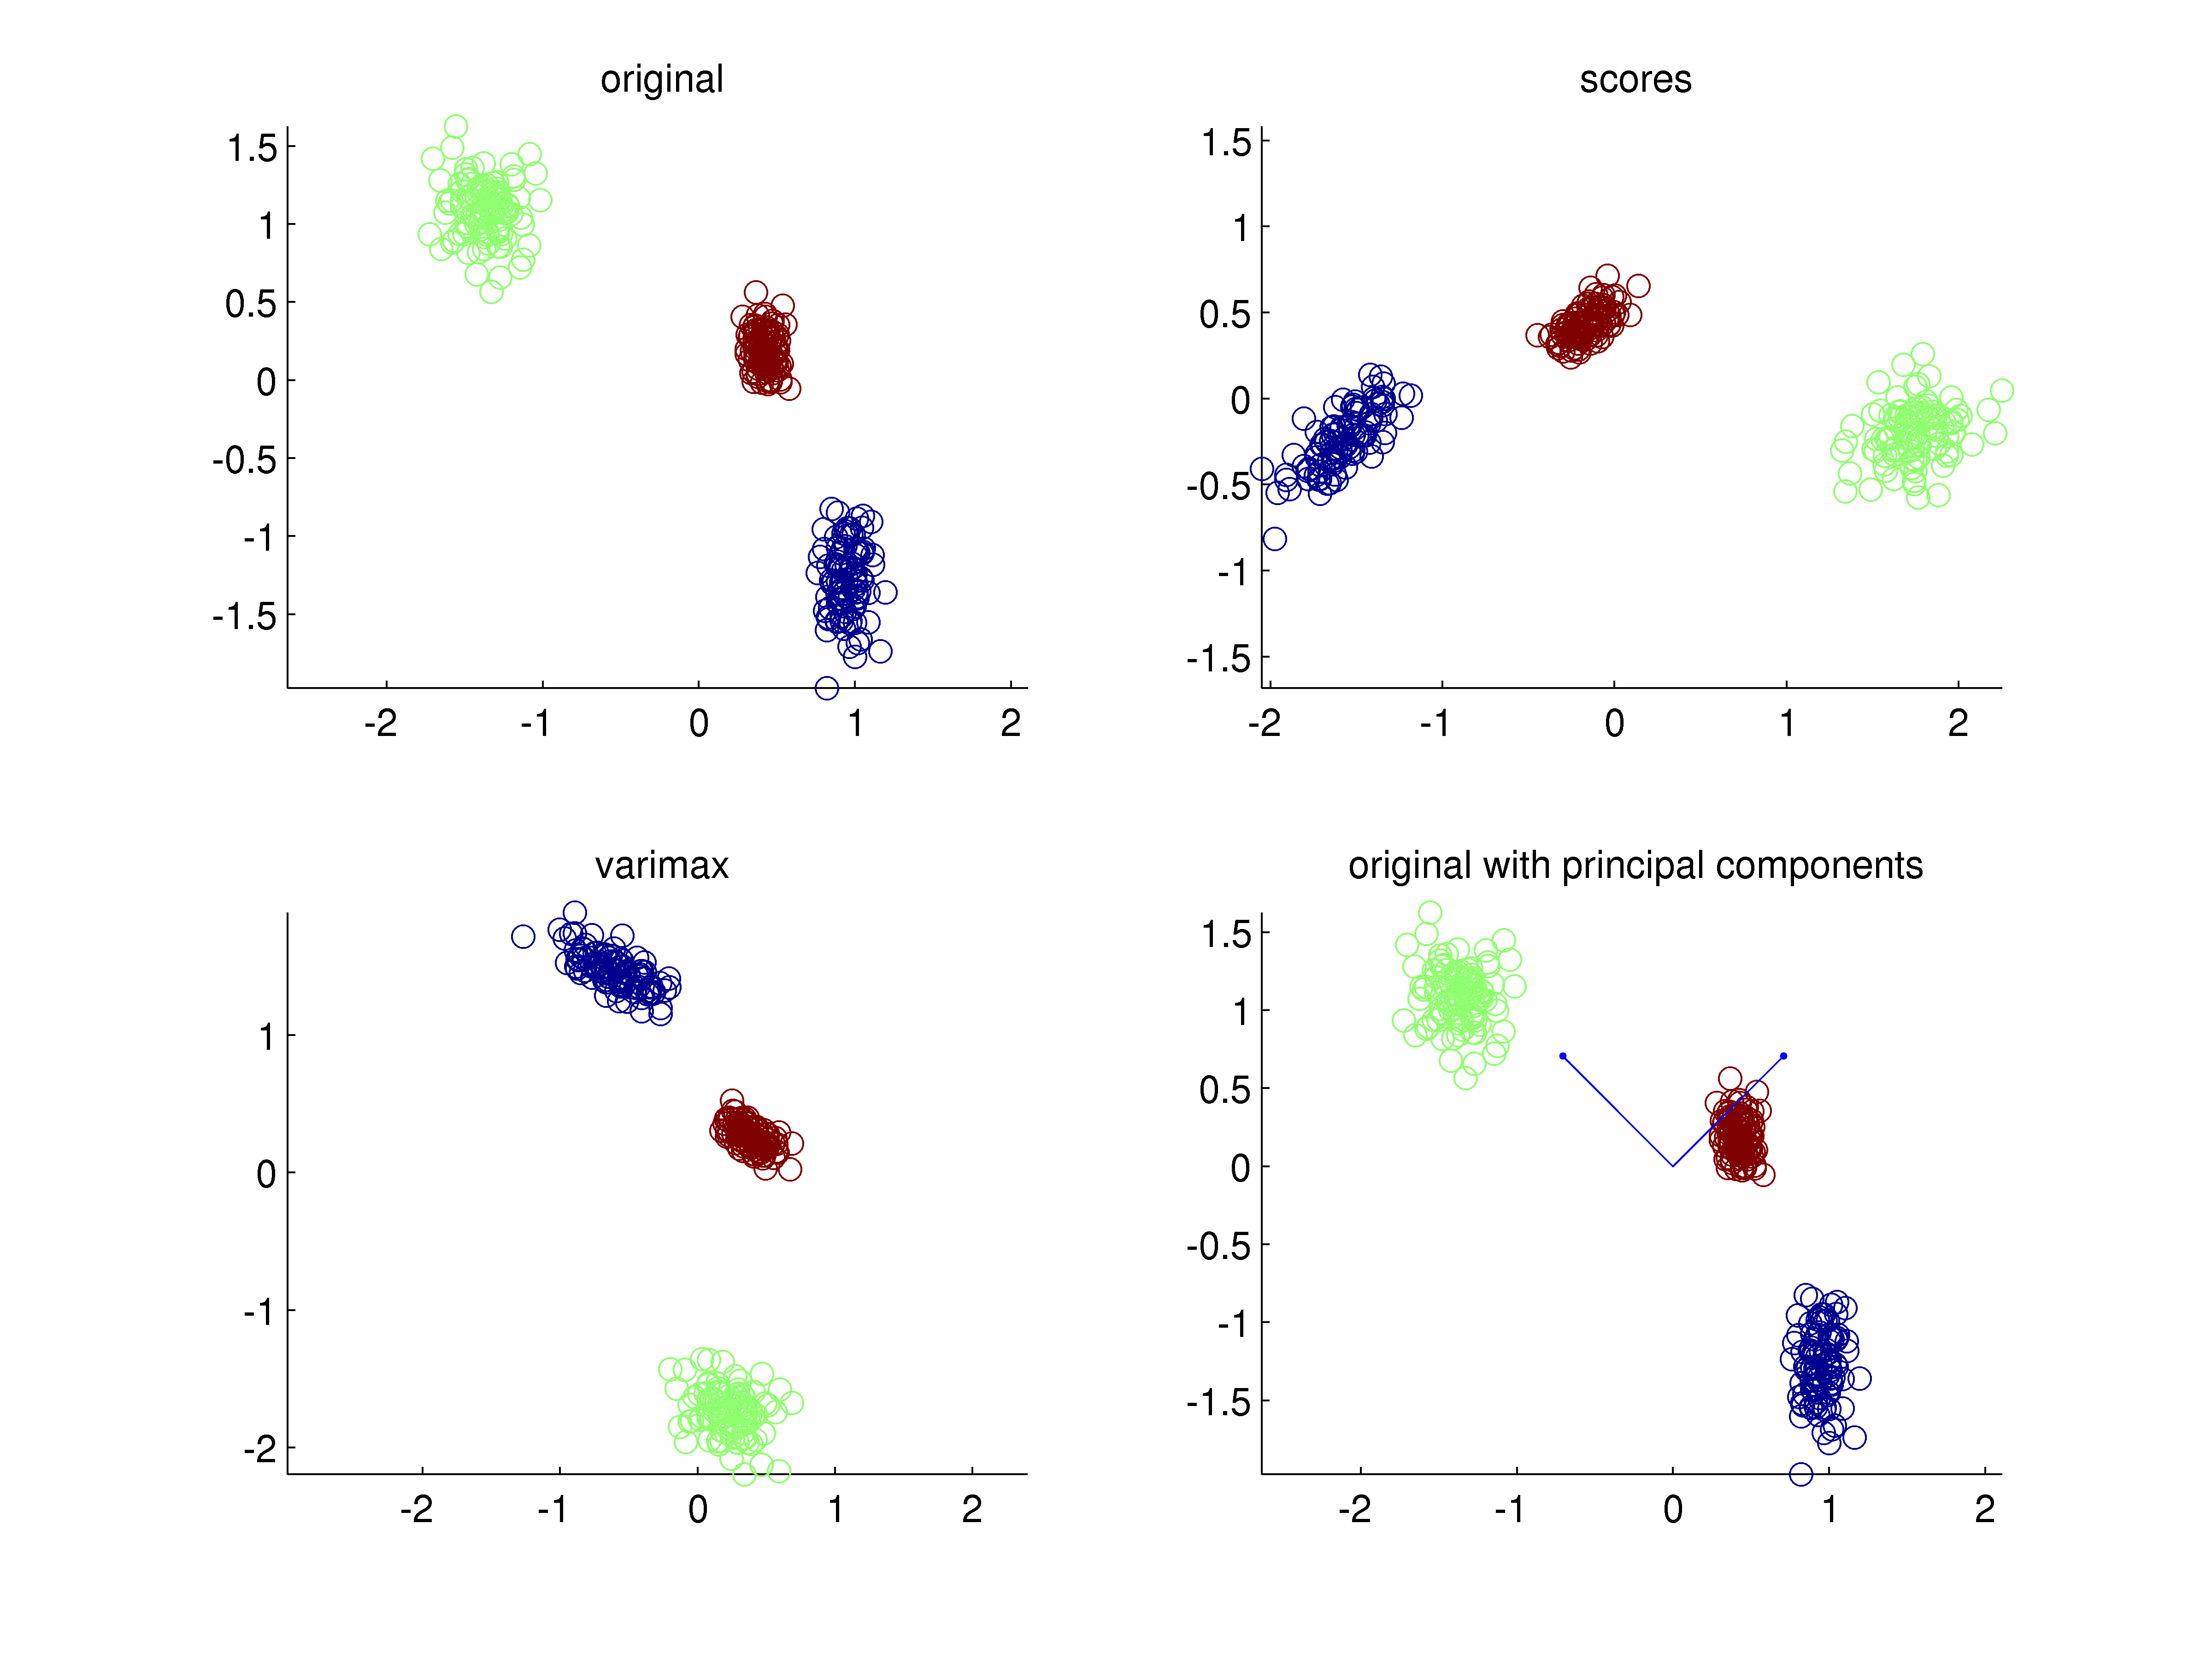
\includegraphics[width=0.9\linewidth]{factor_analysis_rotations}
    \caption{Diagram showing the effect of different rotation methods. 
    \textit{Upper left:} A dataset with three Gaussian clusters. 
    \textit{Upper right:} The scores plot, that is, the original points 
    redrawn in the new, rotated coordinate system of their principal 
    components \textit{Lower left:} The same points after varimax rotation. 
    \textit{Lower right:} The points drawn as they were
    in the original but with the principal components superimposed as arrows.}
    \label{fig:pcarotation}
\end{figure}

If you define a good summary as ``one which captures most of the variability'',
use a linear relationship, and measure variability as
variance then PCA is frequently your first step in factor analysis.
PCA finds a new set of axes for a set of input vectors so that the first
axis captures the most variance, the second is aligned with the direction with 
the second most variance and so forth. These new axes are the principal 
components of the input dataset and all of them are perpendicular to each other.

Figure \ref{fig:pcarotation} displays
graphically the effect of PCA. The upper left shows the original data. The
lower right shows the principal components derived from that data. Finally,
the upper right shows the original data after being rotated so the first
principal component lines up with the horizontal axis. This type of projection 
onto these axes is called a scores plot. It is easy to see that
this new x axis captures more of the spread of the data than either of the 
original two axes. This new axis is a new variable, a single latent factor that 
explains most of the variance in the original data.

Note that though this latent variable model captures an important factor in the 
data, it does not capture all the structure. This data was generated as a 
mixture of three two-dimensional Gaussians, so a perfect model would involve 20 
parameters: the center and covariance matrix for each cluster and the 
probability of generating a point in that cluster\footnote{The center and 
covariance matrix together are 6 parameters per cluster. This accounts for 18 
parameters. Only two mixing probabilities are needed because the probabilities 
must sum to 1, so the total is 20.}. The model we used is linear but the process 
generating the data is nonlinear.

A common variation on PCA is used to capture the covariance of several 
variables. To motivate this variation, imagine a dataset where one variable 
ranges from 0 to 1,000,000 and the rest from 0 to 1. It is easy to see that just 
choosing the large variable will capture most of the variability. However if you 
are interested in the relationships between the variables, their covariance 
structure, this will be hidden by the poor scaling. The solution to this is to 
z-score normalize all of the variables by subtracting their mean and dividing by 
their standard deviation. In that case the variance of each variable will be 1 
and PCA will pick out the axes with the greatest covariation.

\subsection{PCA and Matrices}

Because PCA performs a rotation, it can be looked at as a matrix factorization. 
It produces two matrices. If the input matrix contains observations (or 
individuals) in the rows and measured variables in the columns, the resulting 
matrices can be characterized as follows. The first matrix is the loadings 
matrix, which has rows that are factors and columns that correspond to 
variables. The second is the scores matrix, which has columns that are factors 
and rows that are observations. 

The scores matrix represents the observations (or individuals) expressed in 
terms of the new latent factor variables. The loadings matrix gives the 
relationship between the original variables and the new factors, allowing one 
to be expressed in terms of the other. It is conventional to write the loadings 
matrix so that the factors are unit vectors to make them a unit basis for the 
new space. The separation into loadings and scores is a matrix factorization 
because if you multiply $scores \times loadings$ you get the original matrix 
back. Further, because the principal components are ordered in terms of variance 
captured, if you choose the first n rows of the loadings matrix and multiply 
them by the first n columns of the scores matrix, you will recover an 
approximation to the original matrix that is the best approximation\footnote{The 
approximation is best in a least-squares sense.} that can be made with n 
underlying dimensions.

\subsection{Interpreting the factors}

\subsubsection{Choosing the matrix}
Though machine learning practitioners will seek principal components merely as 
a dimensionality reduction strategy, in the sciences, factors are sought 
because the seeker wishes to understand the system. This requires interpreting
the factors. Either the scores or the loadings matrices can be used in this 
interpretation. The loadings matrix relates factors to the original variables
and the scores matrix relates factors to the original observations. 

Which matrix is chosen for interpretation depends on whether the analyst can 
extract more meaning from the original variables or the original observations. 
For example if the original experiment matched radio frequency emissions with 
rats from two groups at two different times, ``intensity at 300Hz'' carries less 
semantic information about the question under study than ``rat given placebo at 
time 2'', so the analyst would use the scores matrix. On the other hand, consider 
the case where the observations in the experiment were of random people and the 
variables were ``Is gregarious'' and ``Is helpful.'' ``Is gregarious'' has more 
content relating to personality than ``random subject 2011 - male,'' so the 
analyst would use the loadings matrix.

\subsubsection{Creating the interpretation}

\label{sec:bg:factorinterpretation}
Once the appropriate matrix has been chosen, one can use the factors directly
and just look at the highest loading/scoring components (as was done in 
\citep{Samsonovich2010}). However, it is
also common to rotate the factors according to a criterion that makes 
interpretation easier - for example, varimax rotation. Thresholds for a 
significant loading/score are also used. At the end, the analyst has for each
factor a list of items (variables or observations) that are highly ranked for a 
factor and a list that rank poorly on that factor. Based on the meaning of the 
two groups, the analyst can hypothesize what differentiates them that could also
be reflected in the original data and then assign that interpretation to the 
factor.

\section{Lexical Hypothesis in Personality Psychology}

After the \modelname{} model and factor analysis, the third piece of background
crucial to understanding my work is the lexical hypothesis in personality 
psychology.

As mentioned in Section \ref{sec:personalitymodelsfromvectors} there are many
methods for formulating personality models. One approach is to attempt to extract the 
intuitive personality model held by most people. It can be assumed that this
model is reasonably good because our species, being very social, needs to 
interact with and model others as a condition of survival. 

A good way to try and get at this model is to use language. The lexical 
hypothesis in psychology is:
``those individual differences that are most salient and socially relevant in
people's lives will eventually become encoded into their language'' 
\citep[p. 204]{Goldberg1982} This approach was initially proposed by 
Galton \citep[p. 181]{Galton1884} and was pursued by psychologists for the following century
but it made its most significant gains in popularity after an influential seminar
by Goldberg in 1983. \citep[p. 90]{Deary2009}

\subsection{Word lists}

As stated, the lexical hypothesis covers the encoding of personality traits in
all of language. However, as implied by its name, psychologists working from 
the lexical hypothesis have focused on finding personality in the vocabulary
of the language rather than in its grammatical structure. 
\citep[p. 181]{Galton1884} pioneered this
as well, spending time with Roget's Thesaurus and coming back with an estimate
of 1,000 applicable words.

The next notable advance in word lists was reported by Allport and Odbert 
\citep{Allport1936} who tabulated all the trait names in the
Webster's unabridged New International Dictionary. By their count, there were
17,953 terms. They chose words that had the ``capacity ... to distinguish 
the behavior of one human being from that of another.'' Thus, they excluded
words which specified non-distinctive behavior. Because they were
mainly attempting to create a list in which the entries could be rough proxies
for traits, they attempted to reduce redundancy by avoiding nominative and
adverbial forms and including multiple words from clusters where they judged 
that the different forms arose because of arbitrary morphological development 
rather than reflecting semantic distinction. Thus \textasciitilde 18,000 terms, frequently taken to 
be an approximation
of the number of personality terms in the English language is actually an
underestimate.

Allport and Odbert divided their list into 4 categories. The first was the
closest embodiment of the most clearly ``real'' traits of personality. ``They
designate generalized and personalized determining tendencies - consistent and
stable modes of an individual's adjustment to his environment.'' The other three
categories included words that were more temporary, more censorial, and more
metaphorical and remote in their applicability to personality.\footnote{ 
It is interesting that our automatic software includes as some of its most 
important dimensions ones that could be used to categorize words on two of these
axes.
There is a positive-negative component and a ``frequently applies metaphorically''
component. The lack of a component measuring temporariness is not surprising
since the word-list we used excluded words designating temporary states.}

Word lists of the size generated by Allport and Odbert were too large to use 
with statistical techniques before the advent of computers. So, 
\citep{Cattell1947} manually reviewed the list and chose 35 trait variables he felt
summarized the words in Allport's first category trait list. This list is
notable because Cattell used it to produce his influential 16 factor model
and an independent analysis by Tupes and Christal in 1961 \citep{Tupes1992} is 
the first clear recognition of the five factor model.

The last of the massive, dictionary-derived trait lists was published by W. T. 
Norman in 1967 \citep{Norman1967}. He started with all 4 categories of
Allport and Odbert's list and added all words that ``pertained in any
manner to attributed of persons or their behavior but which were not included 
in the Allport-Odbert list'' from Webster's Third New International Dictionary
Unabridged (1961). Then, in a first culling, a group of four raters removed 
the most obscure words, 
those that were
nebulous and extremely metaphorical, physical aspects of behavior, movements,
location, or of appearance, grooming and dress, and finally those which are
purely evaluative, or qualifiers of degree. Next he
classified the remaining words into 15 categories roughly indexing their
stability/temporariness, formality, commonness, reference to social constructs
\footnote{Words like adversary, helpmate, outcast were high in this category}
and then the 4 categories from the first, rough cull. He kept the stable words
that did not refer to social constructs as his list of 2800 trait words. His
list did not restrict itself to adjectives.

After Norman, people continued to produce word lists for trait evaluation. But
many of them were much smaller \textendash designed for use in direct personality 
assessment and they are frequently dependent on one of the earlier lists. We
use two such lists from Goldberg in our later analysis. 
\citep{Saucier1996,Goldberg1990} 

\subsection{Factor-analytically derived traits}

The lexical hypothesis is one of the most important hypotheses in personality
modeling today. But to be useful, the information about personality structure
cannot remain diffused throughout lists of personality words but must be 
extracted and condensed. Starting with Cattell in the 1940's 
\citep[e.g.][]{Cattell1946,Cattell1948} research psychologists turned to factor analysis to 
concentrate the information about personality contained in language into usable
knowledge.

The general method for producing a list of traits through factor analysis is to
measure many variables which one believes are related to personality. Then,
factor analysis will produce clusters of variables that score high or 
low\footnote{usually a cut-off of 
$\left|v\right| > 0.3$ or $\left|v\right| > 0.4$
is chosen for high/low loadings, which means between 9 and 16 percent of the
variance of that variable is accounted for by that factor.} on
a particular factor. These are then used to help the experimenter interpret
that factor as a trait summarizing an important aspect of personality. 
A large majority of studies on personality models 
refer to the Big Five structure \citep[p. 127]{DeRaad2009} which was
derived from just such a factor-analytical approach to the lexical hypothesis.

\chapter{Related Work}

\section{\modelname{} model}

There has not been a lot of time since the publication of the \modelname{} model. 
However, in that period, researchers have attempted to improve its algorithms
and vector quality, and also created applications, both within and outside 
Natural Language Processing (NLP). It has also seen use as a 
standard reference to which the performance of other algorithms is compared.

\subsection{Algorithm and Vector Improvements}

\citep{Mikolov2013c} tested alternative training procedures. They tested an 
alternative to the hierarchical softmax used in the \modelname{} model called 
negative sampling. The also tested a way of giving less weight to frequent words
which speeds up training. The weight adjustment improved the resulting vectors
more than negative sampling. They also demonstrated a simple method
of extracting phrases whose meanings were not simple compositions of their
component part meanings and extended their semantic test suite to use some
of these phrases.

\citep{Faruqui2014} created a method using Canonical Correlation Analysis (CCA) 
to take vectors generated on monolingual corpora for different languages and 
combine them to create new sets of vectors utilizing the semantic information 
from both. They then compared the semantic distance mappings thus obtained to 
several sets of human-labeled semantic distances. They also used the analogy 
tasks from \citep{Mikolov2013a}. With LSA as the source for the original 
vectors, they were able to uniformly improve performance on all measures. 
Similarly, with a Recursive Neural Network (RNN) as the source of the vectors, 
there was less improvement, but still only a loss on one task. Vectors from 
\modelname{} however had no detectable change in most cases but their 
performance decreased on the same task as the RNN\footnote{The authors do not 
mention having done multiple test correction, so their significance values may 
be invalid.}.

\citep{Wolf} also created an extension of \modelname{}\footnote{They use the
CBOW architecture rather than the Skip-gram variation I
use.} that takes advantage of
bilingual information to to improve vector quality. They believe it works 
because it deals better with polysemy, since it is rare that homographs of 
translations cover the same set of senses. They require a word-aligned 
training corpus and use a vocabulary 
composed of all words in both languages. They first train the model on both
languages as usual. Then, they train the words using the context from the 
matched opposite language word. So, for example, the word 
``ran'' is aligned with the word ``corri\'o'' in the two parallel sentences 
``She ran to the store'' and ``Ella corri\'o' a la tienda''. So the context of 
``ran'' in the second phase would be ``Ella,'' ``a,'' ``la,'' and ``tienda.''
\footnote{Because their Hebrew-English parallel text pairs the 
Hebrew Bible with its King James translation, one of their tests involves 
synonyms taken from Strong's 1890 
concordance. Many people believe that
all the senses of a word are expressions of some ``root meaning'' of that word 
and so
pick and choose glosses from Strong's dictionary to give other nuances they 
believe were held by the 
original Greek or Hebrew that did not make it into English. This makes 
Strong's work an ironically appropriate choice for this study 
since this ``root meaning'' assumption is almost the same as the assumption that 
vector-space language models impose by assuming a single point for each word 
and which the authors are trying to overcome by using multiple languages.}

\citep{Bordes2013} extended the implicit linear operators expressing 
relationships in \citep{Mikolov2013b} and explicitly trained a vector
space representation of RDF-type triples 
$(subject,predicate,object)$ that 
capture the semantics of $predicate$ by attempting to make 
$subject+predicate \approx object$ when the predicate holds and make it
far away otherwise. The resulting model is able to predict links better than
several more expressive models by the same authors on both Freebase and 
WordNet datasets. And even when the link predictions do not contain the best
answer, they reflect common sense.

\subsection{Applications}

\citep{Mikolov2013a} creates a method of generating phrase tables and 
dictionaries from two languages with only a small amount of bilingual data.
They first train the \modelname{} model on two independent monolingual corpora 
and then align the vector spaces with a linear transformation derived from a 
small number of matched word pairs. The resulting translations had the 
correct word within the top 5 candidates (which were usually synonyms) 90\% of 
the time.

\citep{Frome2013} used \modelname{} vectors as the targets in a second round
of training a state-of-the-art image recognition convolutional neural network.
The semantic generalization afforded by the vector space structure allowed them
to predict labels for images where it had never seen an image with that label
at all\footnote{There were 1000 labels in the training set and 20,841 unseen 
labels not included in the training set images.}. Later, almost the same team 
published \citep{Norouzi2013} which 
generalized the method to allow use of any n-way image classifier and to 
remove the requirement that the classifier had to be retrained using the 
new output structure. 

\citep{Perozzi2014} created an algorithm called DeepWalk which uses
\modelname{} to assign representations to nodes in a network graph. First, 
random walks on the graph starting at a given node are generated. Each node is
treated as a word and each walk is treated as a sentence. These are then run
through the \modelname{} algorithm to produce vectors that describe each node.
Despite the fact that the vectors are generated using only local information
about the graph, on multi-label classification problems they were able to 
outperform competing techniques that required
a global view of the network - with the competitive advantage increasing with 
the sparsity of the labeled training data. They proposed an on-line version of
the algorithm and one that could capture additional relationships by looking at
non-random paths through the network generated by users.


\citep{Osendorfer2013} proposed using \modelname{} vectors in an information
retrieval setting for computing similarity between musical pieces. Looking at 
music as a language, they intend to use the sparse translation technique from
\citep{Mikolov2013a} to translate between normal language and music.

\section{Studies involving both topic models and personality}

To my knowledge, no one has yet attempted to derive the structure of personality
words by looking at the components of a vector-space model. And 
I am certain no one
has attempted it with vectors from the \modelname{} model. 
However, that does not
mean that the subjects of vector-space lexical semantics and personality are
completely disjoint. I located a number of articles where both played a role.
Most were attempts to predict personality or some aspect thereof from some body 
of text like emails or tweets. There was also one paper that used topic
models as an exploratory tool, attempting to discover more about personality.
A final paper, in deriving results about the structure of language,
found three dimensions that were consistent across different
languages and different source corpora. Of these three, at least two and 
possibly all are personality-relevant.

\subsection{Personality predictive models}

The majority of papers looking at both vector-space language models and 
personality are attempts to predict personality or some aspect thereof from a 
body of text.

\citep{Shen2013} build a classifier to predict three levels
(high, medium, and low) of each of the Big Five personality dimensions from
individual emails using hand-selected features. One of the underlying 
probabilistic models they reject is an LDA variant. Their final classifier
achieves around 70\% accuracy.

\citep{Hill2001} use LSA on a collection of design documents
to produce vectors which they separate into components one coming from 
the author's, speaking personality and the other from the topic of the document.

In \citep{Gill2007} the authors attempted to predict personality using three 
different vector space lexical semantic models including LSA. These models were 
trained on several standard news and academic corpora. They had emails from 
students who had taken the Eysenck Personality Questionnaire and tried to 
predict their extroversion and neuroticism by looking at the similarity of their 
emails to 10 prototypical words ``defining a trait'' from \citep{Goldberg1992} 
and by looking at the 7 words that were most frequent in emails from the people 
who were most extreme on the given traits. The semantic models failed on both 
counts while human raters were able to reliably predict both extroversion and 
neuroticism from the same texts. They concluded that topic models do not extract 
the right kind of information to classify personality. An external observer, 
however, might note their unsophisticated use of pre-made topic models created 
in a different domain to examine poorly selected features in a very small list 
of documents as an alternate explanation for their failure.

In \citep{Arvidsson2011} they use LSA to show that psychotherapy causes changes 
in a self-report-based personality index based on a patient's description of 
himself, his mother and his father. \footnote{I was unable to access the full 
text of this article before I had to submit the thesis but I still felt that the 
article was likely relevant.}

\citep{Pennacchiotti2011} uses a large number of features including topics
from different LDA models to predict various features of Twitter users including
political orientation, which may be considered a correlate of the openness
personality dimension.

\subsection{Questions in the study of personality}

Besides these predictive studies, one article used vector-space lexical 
semantics as a tool to explore personality. \citep{Schwartz2013a} use a database 
of 14.3 million posts from 75,000 Facebook users who took a Five Factor 
questionnaire and analyzed their Facebook posts to gain insight into gender, 
age, and personality. One of the features they examine is topics from an LDA 
model. Their personality-sorted results mainly looked at N-grams (which produced 
the novel observation that introverts like Japanese culture). Their insights 
from the LDA were mainly about lifespan issues. For example, social topics 
increase with age and antisocial topics decrease.

\subsection{Serendipitously discovered personality factors}

Possibly the most relevant work is \citep{Samsonovich2010} (which is an 
expansion of \citep{Samsonovich2007}). In this work the authors are not 
intending to discover anything about personality, rather they are investigating 
the semantic structure of language. They analyze synonyms and antonyms in 
English, French, and German. In all three languages, they discovered that the 
first three principal components could be summarized as measuring 
positive/negative (valence), strong/weak (dominance,arousal), and open/closed 
(freedom). They used a similar criterion to Mikolov for constructing the space 
in that they minimized a cosine distance for close words. But because of the 
presence antonym information, they were also able to specify that antonyms 
should have maximum cosine distance. The resulting vector assignments had 4 
obvious and strong principal components, of which 3 were replicated across 
languages. Because of the underlying human-generated synonym-antonym 
classification, the generated categories better reflect the way humans divide up 
the world. Additionally, the first two categories are similar to several 
two-factor personality models: Morality/Dynamism \citep{Saucier2005} or 
Virtue/Dynamism \citep{DeRaad2008}. The authors also see a similarity between 
their factors and Communion/Power from the interpersonal Circumplex of Leary 
\citep{Leary1957}. This suggests the interesting possibility that the great 
cross-cultural similarity in personality factors comes in part from the fact 
that humans, the main measuring instrument, classify \textit{everything} along 
these two dimensions. It would be a very interesting follow-up to look at the 
portion of semantic space generated from these thesauri inhabited by personality 
words and see what other dimensions are present when the noise of multiple, 
overlapping topic-areas is removed.
